% ============================================================
% SmartFood — Rapport complet final
% Version V3 : Simplexe selon le cours, graphes dédiés
% ============================================================
\documentclass[12pt,a4paper]{article}

\usepackage[utf8]{inputenc}
\usepackage[T1]{fontenc}
\usepackage[french,provide=*]{babel}
\usepackage[top=2.5cm,bottom=2.5cm,left=2.5cm,right=2.5cm]{geometry}
\setlength{\headheight}{15pt}
\usepackage{lmodern}
\usepackage{textcomp}

% ── Mise en page ───────────────────────────────────────────────────────────
\usepackage{fancyhdr}
\pagestyle{fancy}
\fancyhf{}
\fancyhead[L]{\small\textit{SmartFood — Rapport de projet}}
\fancyhead[R]{\small\textit{2024–2025}}
\fancyfoot[C]{\thepage}
\renewcommand{\headrulewidth}{0.4pt}

% ── Maths ──────────────────────────────────────────────────────────────────
\usepackage{amsmath,amssymb,mathtools}

% ── Tableaux ───────────────────────────────────────────────────────────────
\usepackage{booktabs,array,multirow,longtable}
\usepackage[table,dvipsnames]{xcolor}

% ── Graphiques ─────────────────────────────────────────────────────────────
\usepackage{graphicx,caption,adjustbox}
\usepackage{pdflscape}
\usepackage{pgfgantt}

% ── TikZ ───────────────────────────────────────────────────────────────────
\usepackage{tikz}
\usetikzlibrary{arrows.meta,positioning,shapes.geometric,fit,calc,decorations.pathreplacing,backgrounds}

% ── Boîtes ─────────────────────────────────────────────────────────────────
\usepackage[most]{tcolorbox}
\tcbuselibrary{skins,breakable}

% ── Listes ─────────────────────────────────────────────────────────────────
\usepackage{enumitem}

% ── Code ───────────────────────────────────────────────────────────────────
\usepackage{listings}

% ── Typo ───────────────────────────────────────────────────────────────────
\usepackage{microtype,setspace}
\onehalfspacing

% ── Liens ──────────────────────────────────────────────────────────────────
\usepackage[hidelinks,colorlinks=true,linkcolor=BrickRed,urlcolor=NavyBlue]{hyperref}

% ── Couleurs ───────────────────────────────────────────────────────────────
\definecolor{critcolor}{RGB}{231,76,60}
\definecolor{starcolor}{RGB}{52,152,219}
\definecolor{acpmcolor}{RGB}{39,174,96}
\definecolor{headerbg}{RGB}{44,62,80}
\definecolor{pivotcol}{RGB}{255,243,205}
\definecolor{pivotrow}{RGB}{209,250,229}
\definecolor{pivotelt}{RGB}{255,206,84}
\definecolor{codebg}{RGB}{248,249,250}
\definecolor{pyblue}{RGB}{0,0,200}
\definecolor{pygreen}{RGB}{0,150,0}
\definecolor{pygray}{RGB}{120,120,120}
\definecolor{finalized}{RGB}{225,225,225}
\definecolor{pathA}{RGB}{39,174,96}      % vert pour client A
\definecolor{pathB}{RGB}{52,152,219}     % bleu pour client B
\definecolor{pathC}{RGB}{230,126,34}     % orange pour client C
\definecolor{pathD}{RGB}{142,68,173}     % violet pour client D

% ── Environnements boîtes ──────────────────────────────────────────────────
\newtcolorbox{resultbox}{enhanced,breakable,colback=green!8,colframe=acpmcolor!70,
  boxrule=0.8pt,arc=4pt,left=6pt,right=6pt,top=5pt,bottom=5pt,fontupper=\small}
\newtcolorbox{alertbox}{enhanced,breakable,colback=orange!10,colframe=orange!70,
  boxrule=0.8pt,arc=4pt,left=6pt,right=6pt,top=5pt,bottom=5pt,fontupper=\small}
\newtcolorbox{warnbox}{enhanced,breakable,colback=red!8,colframe=critcolor!80,
  boxrule=0.8pt,arc=4pt,left=6pt,right=6pt,top=5pt,bottom=5pt,fontupper=\small}
\newtcolorbox{etape}{enhanced,breakable,colback=blue!4,colframe=starcolor!70,
  boxrule=0.8pt,arc=4pt,left=6pt,right=6pt,top=5pt,bottom=5pt,fontupper=\small,
  title={Étape},coltitle=white}

% ── Style listings ─────────────────────────────────────────────────────────
\lstset{
  language=Python,
  basicstyle=\tiny\ttfamily,
  keywordstyle=\color{pyblue}\bfseries,
  commentstyle=\color{pygreen}\itshape,
  stringstyle=\color{orange!80!black},
  numberstyle=\tiny\color{pygray},
  numbers=left, numbersep=6pt,
  backgroundcolor=\color{codebg},
  frame=single, framesep=4pt, rulecolor=\color{gray!40},
  breaklines=true, breakatwhitespace=true,
  showstringspaces=false,
  columns=fullflexible,
  keepspaces=true,
  literate=
    {é}{{\'{e}}}1 {è}{{\`{e}}}1 {ê}{{\^{e}}}1 {ë}{{\"e}}1
    {à}{{\`{a}}}1 {â}{{\^{a}}}1 {ä}{{\"a}}1
    {ô}{{\^{o}}}1 {ö}{{\"o}}1
    {î}{{\^{i}}}1 {ï}{{\"i}}1
    {ù}{{\`{u}}}1 {û}{{\^{u}}}1 {ü}{{\"u}}1
    {ç}{{\c{c}}}1 {É}{{\'{E}}}1 {È}{{\`{E}}}1 {À}{{\`{A}}}1,
  xleftmargin=1.5em
}

% ── Commandes utiles ──────────────────────────────────────────────────────
\newcommand{\Pred}{\mathrm{Pred}}
\newcommand{\Succ}{\mathrm{Succ}}
\newcommand{\fin}[1]{\cellcolor{finalized}#1}
\newcommand{\sel}[1]{\fbox{\textbf{#1}}}

% =========================================================================
\begin{document}
% =========================================================================

% ── Page de garde ──────────────────────────────────────────────────────────
\begin{titlepage}
\thispagestyle{empty}
\begin{tikzpicture}[remember picture,overlay]
  \fill[headerbg] (current page.north west) rectangle ([yshift=-4.5cm]current page.north east);
  \fill[critcolor] ([yshift=-4.5cm]current page.north west) rectangle ([yshift=-4.9cm]current page.north east);
\end{tikzpicture}
\vspace*{1.8cm}
\begin{center}
  {\color{white}\fontsize{30}{36}\selectfont\bfseries SmartFood}\\[0.3cm]
  {\Large École Nationale Supérieure Polytechnique de Yaoundé - Département du Génie Informatique - 4GI}
\end{center}
\vspace{2cm}
\begin{center}
\begin{tcolorbox}[enhanced,width=0.78\textwidth,colback=white,colframe=headerbg,
  boxrule=1.2pt,arc=6pt,top=12pt,bottom=12pt]
  \centering
  {\Large\bfseries Rapport de projet}\\[0.4em]
  {\huge\bfseries SmartFood}\\[0.4em]
  {\large Optimisation combinatoire, graphes et programmation linéaire}
\end{tcolorbox}
\end{center}
\vspace{1.2cm}
\begin{center}
\begin{tabular}{ll}
\toprule
\multicolumn{2}{c}{\textbf{Équipe — Groupe 12}}\\
\midrule
BELEKOTAN II JEFF NICHOSS         & 24P765 \\
TAGNE SOUOP THOMAS DISNEY         & 22P238 \\
MAGNE ISABELLE CHRIST             & 22P380 \\
FOFACK HENRI                      & 22P231 \\
TOMO MBIANDA ANGELA KATIA         & 22P563 \\
ELOUNDOU NGOUMA THOMAS            & 22P294 \\
AYISSI NGONO ODILE Marie Ange     & 24P764 \\
WATON JEUTA IVANA                 & 24P763 \\
NZIELEU NGNOULAYE NATHAN MAGDIEL  & 22P587 \\
WOKMENI RAISSA                    & 22P246 \\
ZUCHUON KOUGANG NATHANAEL MICHEL  & 22P218 \\
BISSECK CHALVI NATHANAEL          & 22P600 \\
\bottomrule
\end{tabular}
\end{center}
\vfill
\begin{center}{\large Supervisé par : Dr TIONING}\end{center}
\begin{center}{\large Année universitaire 2025–2026}\end{center}
\end{titlepage}

\pagenumbering{roman}
\setcounter{page}{1}
% =========================================================================
\section*{Résumé}
\addcontentsline{toc}{section}{Résumé}
% =========================================================================

Ce rapport présente une étude d'optimisation opérationnelle appliquée à SmartFood,
une entreprise de préparation et livraison de repas. Quatre problèmes de recherche
opérationnelle sont traités : les plus courts chemins par l'algorithme de Dijkstra,
le câblage fibre optique à coût minimal par l'algorithme de Kruskal, l'ordonnancement
de la production par la méthode PERT/Gantt, et la maximisation de la marge quotidienne
par la programmation linéaire (méthode du simplexe). Les résultats montrent que le
trajet optimal vers le client~$A$ est de 10~km, que l'arbre couvrant économise 85~km
par rapport à une étoile naïve, que la durée totale de production est de 158~min avec
un chemin critique de 7~tâches, et que la marge maximale s'établit à 690~\texteuro{}/jour.

\bigskip
\noindent\textbf{Mots-clés :} recherche opérationnelle, Dijkstra, Kruskal, PERT,
programmation linéaire, simplexe, optimisation combinatoire.

\newpage

% =========================================================================
\section*{Abstract}
\addcontentsline{toc}{section}{Abstract}
% =========================================================================

This report presents an operational optimization study applied to SmartFood, a meal
preparation and delivery company. Four operations research problems are addressed:
shortest paths using Dijkstra's algorithm, minimum-cost fiber optic cabling using
Kruskal's algorithm, production scheduling using the PERT/Gantt method, and daily
margin maximization using linear programming (simplex method). Results show that the
optimal route to customer~$A$ is 10~km, the spanning tree saves 85~km compared to a
naive star topology, the total production duration is 158~min with a 7-task critical
path, and the maximum daily margin is 690~\texteuro{}.

\bigskip
\noindent\textbf{Keywords:} operations research, Dijkstra, Kruskal, PERT, linear
programming, simplex, combinatorial optimization.

\newpage


\thispagestyle{empty}
\tableofcontents
\newpage
\listoffigures
\newpage
% =========================================================================
\section*{Liste des abréviations}
\addcontentsline{toc}{section}{Liste des abréviations}
% =========================================================================

\begin{description}[leftmargin=3.5cm, labelwidth=3cm, font=\bfseries]
  \item[ACPM]  Arbre Couvrant de Poids Minimal
  \item[CPM]   \textit{Critical Path Method} — Méthode du Chemin Critique
  \item[MO]    Main-d'\oe{}uvre
  \item[MPM]   Méthode des Potentiels Métra
  \item[PCC]   Plus Court Chemin
  \item[PERT]  \textit{Program Evaluation and Research Task}
  \item[PL]    Programmation Linéaire
  \item[UF]    Union-Find (structure de données)
  \item[$ES$]  \textit{Earliest Start} — Date de début au plus tôt
  \item[$EF$]  \textit{Earliest Finish} — Date de fin au plus tôt
  \item[$LS$]  \textit{Latest Start} — Date de début au plus tard
  \item[$LF$]  \textit{Latest Finish} — Date de fin au plus tard
  \item[$MT$]  Marge Totale
\end{description}
% =========================================================================
\newpage
\section*{Glossaire}
\addcontentsline{toc}{section}{Glossaire}
% =========================================================================

\begin{description}[style=nextline, leftmargin=0.5cm]

  \item[\textbf{Arc}]
  Lien orienté entre deux nœuds d'un graphe, portant un poids (distance, coût ou durée).
  Par opposition à une arête (non orientée), un arc définit une direction de parcours.

  \item[\textbf{Arbre couvrant}]
  Sous-graphe connexe et acyclique reliant tous les nœuds d'un graphe non orienté.
  Un arbre couvrant de $n$ nœuds comporte exactement $n-1$ arêtes.

  \item[\textbf{Base (simplexe)}]
  Ensemble des variables dites « basiques » prenant des valeurs non nulles dans une
  solution de base réalisable. À chaque itération du simplexe, une variable entre en
  base et une autre en sort.

  \item[\textbf{Chemin critique}]
  Dans un réseau PERT, séquence de tâches de durée totale maximale reliant le début
  à la fin du projet. Toute tâche critique a une marge totale nulle : un retard sur
  l'une d'elles retarde obligatoirement la fin du projet.

  \item[\textbf{Graphe orienté}]
  Structure mathématique composée de nœuds (sommets) reliés par des arcs dirigés.
  Utilisé ici pour modéliser le réseau routier de SmartFood.

  \item[\textbf{Marge totale}]
  Retard maximal qu'une tâche peut accumuler sans repousser la date de fin du projet.
  Se calcule par $MT_i = LS_i - ES_i$.

  \item[\textbf{Pivot}]
  Dans la méthode du simplexe, élément à l'intersection de la ligne sortante et de
  la colonne entrante. Toutes les lignes du tableau sont mises à jour en fonction de
  cet élément lors de l'opération de pivotage.

  \item[\textbf{Solution de base réalisable}]
  Solution obtenue en posant toutes les variables hors base à zéro et en résolvant
  le système d'équations résultant. Elle est dite réalisable si toutes les valeurs
  sont non négatives.

  \item[\textbf{Tâche fictive}]
  Tâche de durée nulle introduite dans un diagramme PERT pour modéliser une contrainte
  d'antériorité entre deux branches parallèles sans créer de confusion entre événements.

  \item[\textbf{Variable d'écart}]
  Variable $s_i \geq 0$ ajoutée à une contrainte d'inégalité $\leq$ pour la transformer
  en égalité dans la forme standard de la programmation linéaire.

  \item[\textbf{Union-Find}]
  Structure de données gérant une partition d'ensembles disjoints. Utilisée dans
  l'algorithme de Kruskal pour détecter efficacement les cycles lors de la construction
  de l'arbre couvrant.

\end{description}

\newpage

\pagenumbering{arabic}
\setcounter{page}{1}


% =========================================================================
\section*{Introduction}
\addcontentsline{toc}{section}{Introduction}
% =========================================================================

Dans un contexte économique où la rapidité et l'efficacité constituent des avantages
concurrentiels décisifs, les entreprises de restauration et de livraison à domicile sont
confrontées à des défis d'optimisation de plus en plus complexes. La maîtrise des coûts
logistiques, la qualité du service et la rentabilité de la production sont autant de leviers
qui conditionnent la pérennité d'une telle activité.

C'est dans cette optique que s'inscrit le cas de SmartFood, une entreprise spécialisée
dans la préparation et la livraison de repas commandés en ligne. Disposant d'un entrepôt
central, de quatre cuisines satellites et desservant cinq clients distincts, SmartFood doit
quotidiennement relever plusieurs défis interdépendants : optimiser les trajets de
livraison, déployer une infrastructure réseau à moindre coût, ordonnancer efficacement
sa production, et maximiser sa marge commerciale dans le respect de contraintes
opérationnelles.

Ce rapport propose une étude structurée de ces quatre problématiques à travers
l'optimisation mathématique et la recherche opérationnelle. Plus précisément, les
objectifs poursuivis sont les suivants :

\begin{itemize}
  \item \textbf{Plus courts chemins :} déterminer, pour chaque client, le trajet optimal
        depuis l'entrepôt jusqu'au laboratoire de contrôle qualité en passant par une
        cuisine, à l'aide de l'algorithme de Dijkstra ;
  \item \textbf{Arbre Couvrant de Poids Minimal (ACPM) :} concevoir un réseau de fibre
        optique reliant les dix sites de l'entreprise à coût minimal, grâce aux algorithmes
        de Kruskal ou Prim ;
  \item \textbf{Ordonnancement PERT/Gantt :} planifier la production quotidienne en
        identifiant le chemin critique, les marges de chaque tâche et en analysant
        l'impact d'une contrainte de délai ;
  \item \textbf{Programmation linéaire :} modéliser et résoudre le problème de
        maximisation de la marge quotidienne sous contraintes de ressources et de demande.
\end{itemize}

Chacune de ces problématiques fera l'objet d'une modélisation mathématique rigoureuse,
d'une implémentation en Python, puis d'une analyse de sensibilité permettant d'évaluer
la robustesse des solutions obtenues.

\newpage

% =========================================================================
\section{Modélisation mathématique}
% =========================================================================

% ─────────────────────────────────────────────────────────────────────────
\subsection{Plus court chemin (PCC) — Algorithme de Dijkstra}
% ─────────────────────────────────────────────────────────────────────────

\subsubsection{Définition du graphe orienté}

Le réseau logistique de SmartFood est modélisé par un \textbf{graphe orienté valué}
$G = (S, A, v)$ où :
\begin{itemize}[noitemsep]
  \item $S$ est l'ensemble des \textbf{sommets} (sites) :
        $S = \{E,\, C_1, C_2, C_3, C_4,\, A, B, C, D, F,\, \text{Labo}\}$, avec $|S|=11$ ;
  \item $A \subseteq S \times S$ est l'ensemble des \textbf{arcs} orientés,
        un arc $(i,j) \in A$ étant noté $i \to j$ ;
  \item $v : A \to \mathbb{R}^+$ est la \textbf{valuation} (distance en km) associée à
        chaque arc.
\end{itemize}

Pour chaque sommet $s \in S$, on note :
\[
G(s) = \{t \in S \mid (s,t) \in A\} \quad \text{(successeurs de }s\text{)}
\qquad
G^{-1}(s) = \{r \in S \mid (r,s) \in A\} \quad \text{(prédécesseurs de }s\text{)}
\]

\subsubsection{Problème de plus court chemin}

Étant donné le sommet source $x_0 = E$, on cherche, pour chaque sommet $s \in S$,
la \textbf{distance} :
\[
d(x_0,\, s) = \min_{\substack{\text{chemins } \mu \\ \text{de } x_0 \text{ à } s}}
\sum_{(i,j)\in\mu} v(i,j)
\]

Un chemin $\mu = (x_0, x_1, \ldots, x_n)$ est une suite de sommets telle que
$\forall\, k,\; 0 \le k \le n-1 : (x_k, x_{k+1}) \in A$.
La valuation de $\mu$ est $v(\mu) = \sum_{k=0}^{n-1} v(x_k, x_{k+1})$.

\subsubsection{Principe de l'algorithme de Dijkstra}

L'algorithme de Dijkstra s'applique lorsque toutes les valuations sont
\textbf{positives} : $v(i,j) > 0$ pour tout $(i,j)\in A$.
Il construit itérativement un ensemble $M$ de sommets \emph{marqués} (dont la distance
définitive est connue) :

\begin{enumerate}[noitemsep]
  \item \textbf{Initialisation :} $d(x_0)=0$,\; $P(x_0)=\text{nul}$;\;
        $\forall s\neq x_0 : d(s)=+\infty$,\; $P(s)=\text{nul}$;\; $M=\emptyset$.
  \item \textbf{Sélection :} choisir $x\notin M$ tel que $d(x) = \min_{s\notin M} d(s)$
        ; marquer $x$ ($M \leftarrow M \cup \{x\}$).
  \item \textbf{Relaxation :} pour tout $y \in G(x)$, $y \notin M$ :
        \[
          \text{si}\quad d(x)+v(x,y) < d(y) \quad \Rightarrow \quad
          d(y) \leftarrow d(x)+v(x,y),\quad P(y) \leftarrow x
        \]
  \item Répéter jusqu'à $\min_{s\notin M} d(s) = +\infty$.
\end{enumerate}

La reconstruction du plus court chemin de $x_0$ à $s$ se fait en remontant le
\textbf{tableau des pères} $P$ depuis $s$.

% ─────────────────────────────────────────────────────────────────────────
\subsection{Arbre Couvrant de Poids Minimal (ACPM) — Algorithme de Kruskal}
% ─────────────────────────────────────────────────────────────────────────

\subsubsection{Définition du graphe non orienté}

Le réseau de câblage fibre optique est modélisé par un \textbf{graphe non orienté valué}
$G = (S, A, w)$ avec :
\begin{itemize}[noitemsep]
  \item $S$ : ensemble de $n = 10$ sommets (les dix sites SmartFood) ;
  \item $A$ : ensemble d'arêtes $\{i,j\}$, sans orientation ni arcs parallèles ;
  \item $w : A \to \mathbb{R}^+$ : valuation (longueur du câble en km).
\end{itemize}

Le degré d'un sommet $x$ est $d(x) = |\{e \in A \mid x \in e\}|$, et le
\textbf{théorème des poignées de mains} donne $\sum_{x\in S} d(x) = 2|A|$.

\subsubsection{Arbre couvrant de poids minimum}

Un \textbf{arbre couvrant} de $G$ est un sous-graphe couvrant $G'=(S, F)$
($F \subseteq A$) connexe et sans cycle. Tout arbre à $n$ sommets possède
exactement $n-1$ arêtes.

Un \textbf{arbre couvrant de poids minimum} (ACPM) est un arbre couvrant
minimisant la somme des valuations :
\[
\min_{F \subseteq A} \sum_{\{i,j\}\in F} w_{ij}
\quad\text{s.c.}\quad
(S, F) \text{ connexe et acyclique}
\]

\subsubsection{Algorithme de Kruskal (glouton)}

L'algorithme de Kruskal construit l'ACPM de manière gloutonne :

\begin{enumerate}[noitemsep]
  \item \textbf{Initialisation :} $F = \emptyset$ ; trier les arêtes de $A$ par
        valuations croissantes.
  \item \textbf{Itération :} pour chaque arête $e \in A$ (dans l'ordre) :
        \quad si $F \cup \{e\}$ est \emph{acyclique}, alors $F \leftarrow F \cup \{e\}$.
  \item \textbf{Arrêt :} dès $|F| = n-1$ arêtes sélectionnées.
\end{enumerate}

La détection des cycles est assurée efficacement par la structure
\textbf{Union-Find} (union par rang avec compression de chemin).

% ─────────────────────────────────────────────────────────────────────────
\subsection{Ordonnancement PERT/Gantt}
% ─────────────────────────────────────────────────────────────────────────

\subsubsection{Graphe potentiels-tâches (MPM)}

Le problème d'ordonnancement est modélisé par un \textbf{graphe potentiels-tâches}
$G = (S, A, d)$ orienté et valué, conforme à la méthode MPM (Méthode des Potentiels
Métra) :
\begin{itemize}[noitemsep]
  \item chaque \textbf{sommet} $i \in S$ représente une tâche $T_i$, de durée $d_i > 0$ ;
  \item un \textbf{arc} $(i,j) \in A$ traduit une \emph{contrainte d'antériorité} :
        la tâche $i$ doit se terminer avant que $j$ puisse démarrer ;
  \item l'arc $(i,j)$ est valué par $d_i$ (durée d'exécution de $i$) ;
  \item deux sommets fictifs $\text{DEBUT}$ et $\text{FIN}$ (durées nulles) assurent
        un unique point de départ et d'arrivée.
\end{itemize}

L'ensemble des tâches est $\mathcal{T} = \{P_1, P_2, P_3, P_4, L_1, L_2, L_3, L_4\}$.

\subsubsection{Dates au plus tôt (passage avant)}

On note $T_i$ la \textbf{date de début au plus tôt} de la tâche $i$.
Initialisation : $T_{\text{DEBUT}} = 0$.
\[
T_j = \max_{i \in G^{-1}(j)}\bigl(T_i + d_{i,j}\bigr)
\quad\forall j \in S \setminus \{\text{DEBUT}\}
\]

\subsubsection{Dates au plus tard (passage arrière)}

On note $T^*_i$ la \textbf{date de début au plus tard} de la tâche $i$.
Initialisation : $T^*_{\text{FIN}} = T_{\text{FIN}}$.
\[
T^*_i = \min_{j \in G(i)}\bigl(T^*_j - d_{i,j}\bigr)
\quad\forall i \in S \setminus \{\text{FIN}\}
\]

\subsubsection{Marges et chemin critique}

\noindent\textbf{Marge totale} de la tâche $(i,j)$ :
\[
MT_{i,j} = T^*_j - T_i - d_{i,j}
\]
La marge totale représente le retard maximal qu'on peut prendre sur la tâche
$(i \to j)$ \emph{sans retarder la fin du projet}.

\noindent\textbf{Marge libre} de la tâche $(i,j)$ :
\[
ML_{i,j} = T_j - T_i - d_{i,j}
\]
La marge libre représente le retard qu'on peut prendre sans affecter la date
au plus tôt d'aucune tâche suivante.

\noindent\textbf{Chemin critique :} succession de tâches dont toutes les marges
totales sont nulles ($MT = 0$). Tout retard sur une tâche critique retarde
obligatoirement la fin du projet.
\[
\mathcal{C}^* = \bigl\{(i,j) \in A \mid MT_{i,j} = 0\bigr\}
\]

\subsubsection{Diagramme de Gantt}

Parallèlement au graphe PERT, le \textbf{diagramme de Gantt} représente chaque tâche
par un segment horizontal dans un tableau temps/tâches. Chaque ligne correspond à
une tâche, chaque colonne à une unité de temps. La \emph{progression réelle} peut
y être tracée en pointillé pour le suivi d'avancement. Le chemin critique correspond
au chemin le plus long en terme de durées.

% ─────────────────────────────────────────────────────────────────────────
\subsection{Programmation linéaire}
% ─────────────────────────────────────────────────────────────────────────

\subsubsection{Signification des notations}

On considère un problème de programmation linéaire général à $n$ variables de décision
et $m$ contraintes. Les notations sont les suivantes :

\begin{description}[noitemsep, leftmargin=2cm, labelwidth=1.7cm]
  \item[$Z$]      La fonction objectif globale à optimiser
                  (maximiser le profit ou minimiser le coût).
  \item[$x_j$]    La $j$-ème variable de décision, pour $j = 1, 2, \ldots, n$.
  \item[$c_j$]    Le coefficient de profit (ou coût) unitaire lié à la variable $x_j$.
  \item[$b_i$]    Le second membre de la contrainte $i$ (limite de la ressource $i$),
                  pour $i = 1, 2, \ldots, m$.
  \item[$a_{ij}$] Le coefficient technologique : quantité de ressource $i$ consommée
                  par une unité de la variable $x_j$.
\end{description}

\subsubsection{Forme canonique générale (développée)}

Pour $n$ variables de décision et $m$ contraintes, le modèle s'écrit :

\noindent\textbf{Optimiser (Maximiser ou Minimiser) :}
\[
Z = c_1 x_1 + c_2 x_2 + \cdots + c_n x_n
\]

\noindent\textbf{Sous les contraintes (au nombre de $m$) :}
\[
\begin{array}{r@{\;}c@{\;}l}
a_{11}x_1 + a_{12}x_2 + \cdots + a_{1n}x_n & \leq\;(\text{ou}\;\geq,\;=) & b_1 \\
a_{21}x_1 + a_{22}x_2 + \cdots + a_{2n}x_n & \leq\;(\text{ou}\;\geq,\;=) & b_2 \\
\vdots & \vdots & \vdots \\
a_{m1}x_1 + a_{m2}x_2 + \cdots + a_{mn}x_n & \leq\;(\text{ou}\;\geq,\;=) & b_m
\end{array}
\]

\noindent\textbf{Contraintes de non-négativité :}
\[
x_1 \geq 0, \quad x_2 \geq 0, \quad \ldots, \quad x_n \geq 0
\]

\subsubsection{Forme condensée (avec le symbole $\sum$)}

Cette écriture résume le système précédent de manière compacte :

\noindent\textbf{Optimiser :}
\[
Z = \sum_{j=1}^{n} c_j\, x_j
\]

\noindent\textbf{Sous les contraintes :}
\[
\sum_{j=1}^{n} a_{ij}\, x_j \;\leq\; b_i \qquad
\text{pour tout } i \in \{1, 2, \ldots, m\}
\]

\noindent\textbf{Contraintes de non-négativité :}
\[
x_j \geq 0 \qquad \text{pour tout } j \in \{1, 2, \ldots, n\}
\]

\subsubsection{Forme matricielle}

On regroupe les variables et paramètres dans les structures suivantes :
\[
X = \begin{pmatrix} x_1 \\ x_2 \\ \vdots \\ x_n \end{pmatrix}, \quad
C^T = \begin{pmatrix} c_1 \\ c_2 \\ \vdots \\ c_n \end{pmatrix}, \quad
A = \begin{pmatrix}
a_{11} & a_{12} & \cdots & a_{1n} \\
a_{21} & a_{22} & \cdots & a_{2n} \\
\vdots & \vdots & \ddots & \vdots \\
a_{m1} & a_{m2} & \cdots & a_{mn}
\end{pmatrix}, \quad
B = \begin{pmatrix} b_1 \\ b_2 \\ \vdots \\ b_m \end{pmatrix}
\]

\noindent Le modèle compact s'écrit :
\[
\text{Optimiser}\quad Z = C^T X
\qquad
\text{s.c.}\quad AX \leq B, \quad X \geq 0
\]

\subsubsection{Application à SmartFood}

Les variables de décision sont : $x_1 = S$ (repas Standard),
$x_2 = V$ (repas Végétarien), $x_3 = G$ (repas sans Gluten), avec $n = 3$ et
$m = 6$ contraintes de ressources principales.

\medskip
\noindent\textbf{Vecteur des profits unitaires :}
\[
C^T = \begin{pmatrix} c_1 \\ c_2 \\ c_3 \end{pmatrix}
    = \begin{pmatrix} 3 \\ 4 \\ 5 \end{pmatrix}
\quad (\text{en \texteuro/repas})
\]

\noindent\textbf{Matrice des coefficients technologiques et vecteur des disponibilités :}
\[
A = \begin{pmatrix}
a_{11} & a_{12} & a_{13} \\
a_{21} & a_{22} & a_{23} \\
a_{31} & a_{32} & a_{33} \\
a_{41} & a_{42} & a_{43} \\
a_{51} & a_{52} & a_{53} \\
a_{61} & a_{62} & a_{63}
\end{pmatrix}
=
\begin{pmatrix}
0{,}5 & 1{,}0 & 0{,}3 \\
0{,}8 & 0     & 0     \\
0{,}4 & 0{,}6 & 0{,}9 \\
2{,}0 & 1{,}5 & 3{,}0 \\
1{,}5 & 1{,}2 & 2{,}0 \\
1{,}0 & 1{,}0 & 1{,}0
\end{pmatrix}
\qquad
B = \begin{pmatrix} b_1 \\ b_2 \\ b_3 \\ b_4 \\ b_5 \\ b_6 \end{pmatrix}
=
\begin{pmatrix} 100 \\ 80 \\ 120 \\ 480 \\ 600 \\ 200 \end{pmatrix}
\begin{array}{l}
\text{(légumes, kg)}\\
\text{(viande, kg)}\\
\text{(céréales, kg)}\\
\text{(cuisson, min)}\\
\text{(main-d'œuvre, min)}\\
\text{(total repas)}
\end{array}
\]

\noindent\textbf{Formulation complète du modèle (forme développée) :}

\begin{equation}
\label{eq:pl_smartfood}
\boxed{
\begin{aligned}
\max\; &Z = c_1 x_1 + c_2 x_2 + c_3 x_3
          = 3x_1 + 4x_2 + 5x_3 \quad (\text{en \texteuro/jour})\\[6pt]
\text{s.c.}\quad
&a_{11}x_1 + a_{12}x_2 + a_{13}x_3 \leq b_1
 \;\Leftrightarrow\; 0{,}5x_1 + x_2 + 0{,}3x_3 \leq 100
 \quad \text{(légumes)}\\
&a_{21}x_1 \phantom{{}+a_{22}x_2+a_{23}x_3} \leq b_2
 \;\Leftrightarrow\; 0{,}8x_1 \leq 80
 \quad \text{(viande)}\\
&a_{31}x_1 + a_{32}x_2 + a_{33}x_3 \leq b_3
 \;\Leftrightarrow\; 0{,}4x_1 + 0{,}6x_2 + 0{,}9x_3 \leq 120
 \quad \text{(céréales)}\\
&a_{41}x_1 + a_{42}x_2 + a_{43}x_3 \leq b_4
 \;\Leftrightarrow\; 2x_1 + 1{,}5x_2 + 3x_3 \leq 480
 \quad \text{(cuisson)}\\
&a_{51}x_1 + a_{52}x_2 + a_{53}x_3 \leq b_5
 \;\Leftrightarrow\; 1{,}5x_1 + 1{,}2x_2 + 2x_3 \leq 600
 \quad \text{(MO)}\\
&a_{61}x_1 + a_{62}x_2 + a_{63}x_3 \leq b_6
 \;\Leftrightarrow\; x_1 + x_2 + x_3 \leq 200
 \quad \text{(total)}\\[4pt]
&20 \leq x_1 \leq 100, \quad 20 \leq x_2 \leq 80, \quad 20 \leq x_3 \leq 50\\
&x_j \in \mathbb{N}, \quad j = 1, 2, 3
\end{aligned}
}
\end{equation}

\newpage

% =========================================================================
\section{Résultats détaillés}
% =========================================================================

% ─────────────────────────────────────────────────────────────────────────
\subsection{Vue d'ensemble du réseau SmartFood}
% ─────────────────────────────────────────────────────────────────────────

Avant d'entamer la résolution détaillée de chaque problème, présentons le graphe
\textbf{orienté} qui modélise l'ensemble des trajets logistiques de l'entreprise.
Les nœuds représentent les sites (entrepôt $E$, cuisines $C_1$--$C_4$, clients
$A,B,C,D,F$, laboratoire), et les arcs portent les distances en kilomètres.

\begin{center}
\resizebox{0.95\textwidth}{!}{%
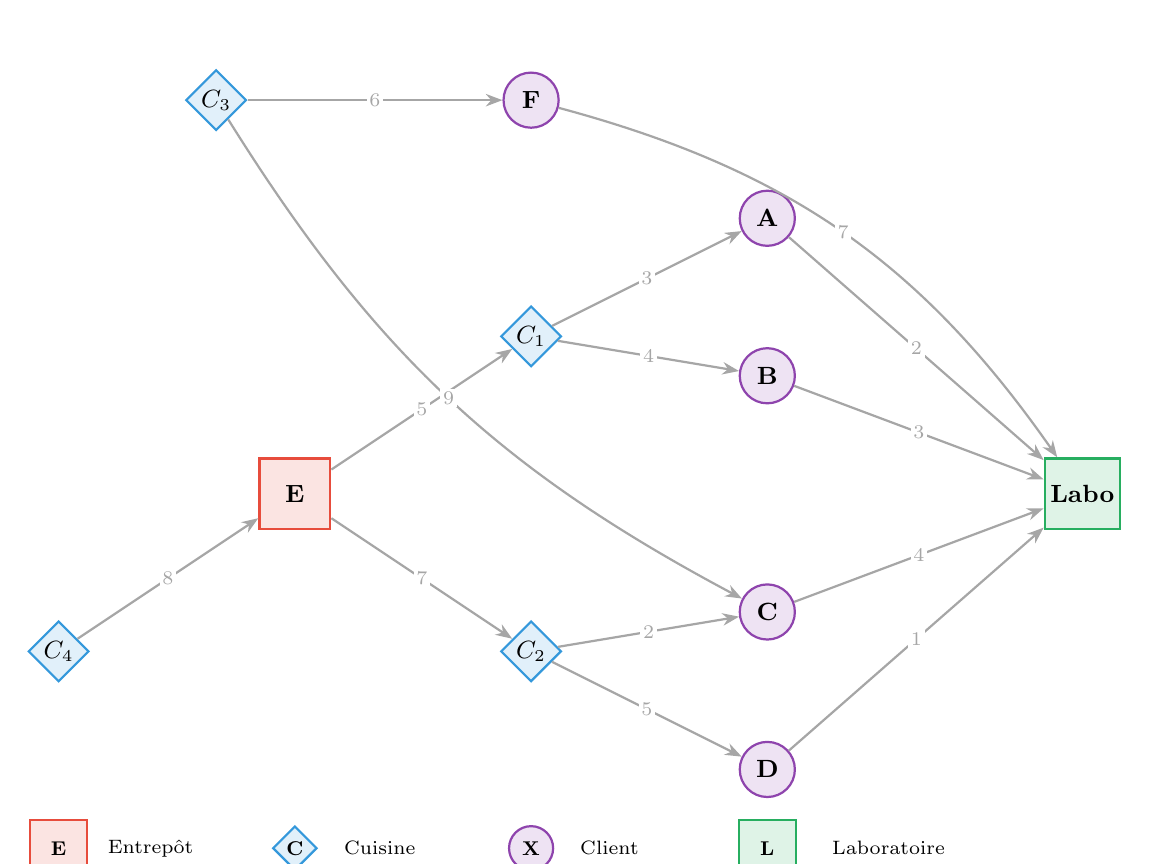
\begin{tikzpicture}[
  >={Stealth[length=6pt]},
  entrepot/.style={rectangle,draw=critcolor,fill=critcolor!15,thick,
                   minimum size=0.9cm,font=\small\bfseries,inner sep=2pt},
  cuisine/.style={diamond,draw=starcolor,fill=starcolor!15,thick,
                  minimum size=0.7cm,font=\small\bfseries,inner sep=1pt},
  client/.style={circle,draw=pathD,fill=pathD!15,thick,
                 minimum size=0.7cm,font=\small\bfseries,inner sep=1pt},
  labo/.style={rectangle,draw=acpmcolor,fill=acpmcolor!15,thick,
               minimum size=0.9cm,font=\small\bfseries,inner sep=2pt},
  arc/.style={->,thick,gray!70},
  lbl/.style={font=\scriptsize,fill=white,inner sep=1pt}
]
%% Nœuds
\node[entrepot] (E)  at (0,0)    {E};
\node[cuisine]  (C1) at (3,2)    {$C_1$};
\node[cuisine]  (C2) at (3,-2)   {$C_2$};
\node[cuisine]  (C3) at (-1,5)   {$C_3$};
\node[cuisine]  (C4) at (-3,-2)  {$C_4$};
\node[client]   (A)  at (6,3.5)  {A};
\node[client]   (B)  at (6,1.5)  {B};
\node[client]   (C)  at (6,-1.5) {C};
\node[client]   (D)  at (6,-3.5) {D};
\node[client]   (F)  at (3,5)    {F};
\node[labo]     (L)  at (10,0)   {Labo};
%% Arcs
\draw[arc] (E)  -- node[lbl]{5}   (C1);
\draw[arc] (E)  -- node[lbl]{7}   (C2);
\draw[arc] (C1) -- node[lbl]{3}   (A);
\draw[arc] (C1) -- node[lbl]{4}   (B);
\draw[arc] (C2) -- node[lbl]{2}   (C);
\draw[arc] (C2) -- node[lbl]{5}   (D);
\draw[arc] (C3) -- node[lbl]{6}   (F);
\draw[arc] (C3) to[bend right=15] node[lbl]{9} (C);
\draw[arc] (C4) -- node[lbl]{8}   (E);
\draw[arc] (A)  -- node[lbl]{2}   (L);
\draw[arc] (B)  -- node[lbl]{3}   (L);
\draw[arc] (C)  -- node[lbl]{4}   (L);
\draw[arc] (D)  -- node[lbl]{1}   (L);
\draw[arc] (F)  to[bend left=20] node[lbl]{7} (L);
%% Légende
\node[entrepot,scale=0.8] at (-3,-4.5) {E};
\node[right,font=\scriptsize] at (-2.5,-4.5) {Entrepôt};
\node[cuisine,scale=0.8] at (0,-4.5) {C};
\node[right,font=\scriptsize] at (0.5,-4.5) {Cuisine};
\node[client,scale=0.8] at (3,-4.5) {X};
\node[right,font=\scriptsize] at (3.5,-4.5) {Client};
\node[labo,scale=0.8] at (6,-4.5) {L};
\node[right,font=\scriptsize] at (6.7,-4.5) {Laboratoire};
\end{tikzpicture}
}
\captionof{figure}{Graphe orienté du réseau SmartFood — distances en km}
\end{center}

\begin{alertbox}
\textbf{Remarque importante :} la cuisine $C_3$ \textbf{n'a aucun arc entrant} depuis $E$
dans le graphe orienté ; le client $F$, dépendant exclusivement de $C_3$, est donc
\textbf{inaccessible} dans le réseau actuel. La cuisine $C_4$, quant à elle, ne pointe
que vers $E$ (arc retour) et ne dessert directement aucun client.
\end{alertbox}

\newpage

% ─────────────────────────────────────────────────────────────────────────
\subsection{Plus court chemin — Dijkstra}
% ─────────────────────────────────────────────────────────────────────────

\subsubsection{Tableau des itérations de Dijkstra}

On applique l'algorithme de Dijkstra depuis la source $x_0 = E$.
La colonne $M$ indique l'ensemble des sommets marqués à chaque étape.
Les distances estimées $d(s)$ sont mises à jour à chaque relaxation (valeur en gras = mise à jour).
Le tableau des pères $P(s)$ est rempli au moment où le sommet est marqué.

\medskip
\noindent\textbf{Initialisation :}
$d(E)=0,\;P(E)=\text{nul}$;\quad
$d(s)=+\infty,\;P(s)=\text{nul}\;\forall s\neq E$;\quad
$M=\emptyset,\;\min\_dist\_M = 0$.

\begin{landscape}
\thispagestyle{fancy}
\vspace*{0.3cm}

\begin{center}
\small\textbf{Application de l'algorithme de Dijkstra — source $x_0 = E$}
\vspace{6pt}

\setlength{\tabcolsep}{5pt}
\renewcommand{\arraystretch}{1.5}
\small
\resizebox{\linewidth}{!}{%
\begin{tabular}{c||c|c|c|c|c|c|c|c|c|c||c|c|c|c|c|c|c|c|c|c}
\hline
\multirow{2}{*}{$M$} &
\multicolumn{10}{c||}{\textbf{Distances estimées}} &
\multicolumn{10}{c}{\textbf{Tableau des pères $P(s)$}} \\
\cline{2-21}
& $d(E)$ & $d(C_1)$ & $d(C_2)$ & $d(C_3)$ & $d(C_4)$ & $d(A)$ & $d(B)$ & $d(C)$ & $d(D)$ & $d(\mathrm{Labo})$
& $P(E)$ & $P(C_1)$ & $P(C_2)$ & $P(C_3)$ & $P(C_4)$ & $P(A)$ & $P(B)$ & $P(C)$ & $P(D)$ & $P(\mathrm{Labo})$ \\
\hline
$\emptyset$ &
\textbf{0} & $+\infty$ & $+\infty$ & $+\infty$ & $+\infty$ & $+\infty$ & $+\infty$ & $+\infty$ & $+\infty$ & $+\infty$ &
nul & nul & nul & nul & nul & nul & nul & nul & nul & nul \\
\hline
$\{E\}$ &
\fin{0} & \textbf{5} & \textbf{7} & $+\infty$ & $+\infty$ & $+\infty$ & $+\infty$ & $+\infty$ & $+\infty$ & $+\infty$ &
nul & $E$ & $E$ & & & & & & & \\
\hline
$\{E,C_1\}$ &
\fin{0} & \fin{5} & 7 & $+\infty$ & $+\infty$ & \textbf{8} & \textbf{9} & $+\infty$ & $+\infty$ & $+\infty$ &
nul & $E$ & $E$ & & & $C_1$ & $C_1$ & & & \\
\hline
$\{E,C_1,C_2\}$ &
\fin{0} & \fin{5} & \fin{7} & $+\infty$ & $+\infty$ & 8 & 9 & \textbf{9} & \textbf{12} & $+\infty$ &
nul & $E$ & $E$ & & & $C_1$ & $C_1$ & $C_2$ & $C_2$ & \\
\hline
$\{E,C_1,C_2,A\}$ &
\fin{0} & \fin{5} & \fin{7} & $+\infty$ & $+\infty$ & \fin{8} & 9 & 9 & 12 & \textbf{10} &
nul & $E$ & $E$ & & & $C_1$ & $C_1$ & $C_2$ & $C_2$ & $A$ \\
\hline
$\{E,C_1,C_2,A,B\}$ &
\fin{0} & \fin{5} & \fin{7} & $+\infty$ & $+\infty$ & \fin{8} & \fin{9} & 9 & 12 & 10 &
nul & $E$ & $E$ & & & $C_1$ & $C_1$ & $C_2$ & $C_2$ & $A$ \\
\hline
$\{E,C_1,C_2,A,B,C\}$ &
\fin{0} & \fin{5} & \fin{7} & $+\infty$ & $+\infty$ & \fin{8} & \fin{9} & \fin{9} & 12 & 10 &
nul & $E$ & $E$ & & & $C_1$ & $C_1$ & $C_2$ & $C_2$ & $A$ \\
\hline
$\{E,C_1,C_2,A,B,C,\mathrm{Labo}\}$ &
\fin{0} & \fin{5} & \fin{7} & $+\infty$ & $+\infty$ & \fin{8} & \fin{9} & \fin{9} & 12 & \fin{10} &
nul & $E$ & $E$ & & & $C_1$ & $C_1$ & $C_2$ & $C_2$ & $A$ \\
\hline
$\{E,C_1,C_2,A,B,C,\mathrm{Labo},D\}$ &
\fin{0} & \fin{5} & \fin{7} & $+\infty$ & $+\infty$ & \fin{8} & \fin{9} & \fin{9} & \fin{12} & \fin{10} &
nul & $E$ & $E$ & — & — & $C_1$ & $C_1$ & $C_2$ & $C_2$ & $A$ \\
\hline
\multicolumn{21}{l}{\textit{$C_3$, $C_4$, $F$ : jamais atteints — $d=+\infty$, $P=$ nul. $\min\_dist\_M = +\infty$ $\Rightarrow$ arrêt.}}\\
\hline
\end{tabular}
}
\end{center}

\vspace{0.5cm}

\noindent\textbf{Reconstruction des chemins} (remontée du tableau des pères) :

\begin{center}\small
\begin{tabular}{c|l|c}
\toprule
\textbf{Client} & \textbf{Chemin (remontée : $s \xleftarrow{P} \cdots \xleftarrow{P} E$)} & \textbf{Distance}\\
\midrule
$A$ & $\mathrm{Labo}\xleftarrow{P(A)}C_1\xleftarrow{P(C_1)}E$
    $\;\Rightarrow\; E\to C_1\to A\to\mathrm{Labo}$ & \textbf{10 km}\\
$B$ & $\mathrm{Labo}\xrightarrow{\text{recalc}}B\xleftarrow{P(B)}C_1\xleftarrow{P(C_1)}E$
    $\;\Rightarrow\; E\to C_1\to B\to\mathrm{Labo}$ & \textbf{12 km}\\
$C$ & $\mathrm{Labo}\xrightarrow{\text{recalc}}C\xleftarrow{P(C)}C_2\xleftarrow{P(C_2)}E$
    $\;\Rightarrow\; E\to C_2\to C\to\mathrm{Labo}$ & \textbf{13 km}\\
$D$ & $\mathrm{Labo}\xrightarrow{\text{recalc}}D\xleftarrow{P(D)}C_2\xleftarrow{P(C_2)}E$
    $\;\Rightarrow\; E\to C_2\to D\to\mathrm{Labo}$ & \textbf{13 km}\\
$F$ & $d(F)=+\infty$ — inaccessible & —\\
\bottomrule
\end{tabular}
\end{center}

\end{landscape}

% ─────────────────────────────────────────────────────────────────────────
\subsubsection{Visualisation des plus courts chemins}
% ─────────────────────────────────────────────────────────────────────────

Le graphe ci-dessous reprend le réseau SmartFood en mettant en évidence, en couleurs
distinctes et en \textbf{trait épais}, les quatre plus courts chemins obtenus pour les
clients $A$, $B$, $C$ et $D$. Le client $F$ apparaît en pointillé gris (inaccessible).

\begin{center}
\resizebox{0.95\textwidth}{!}{%
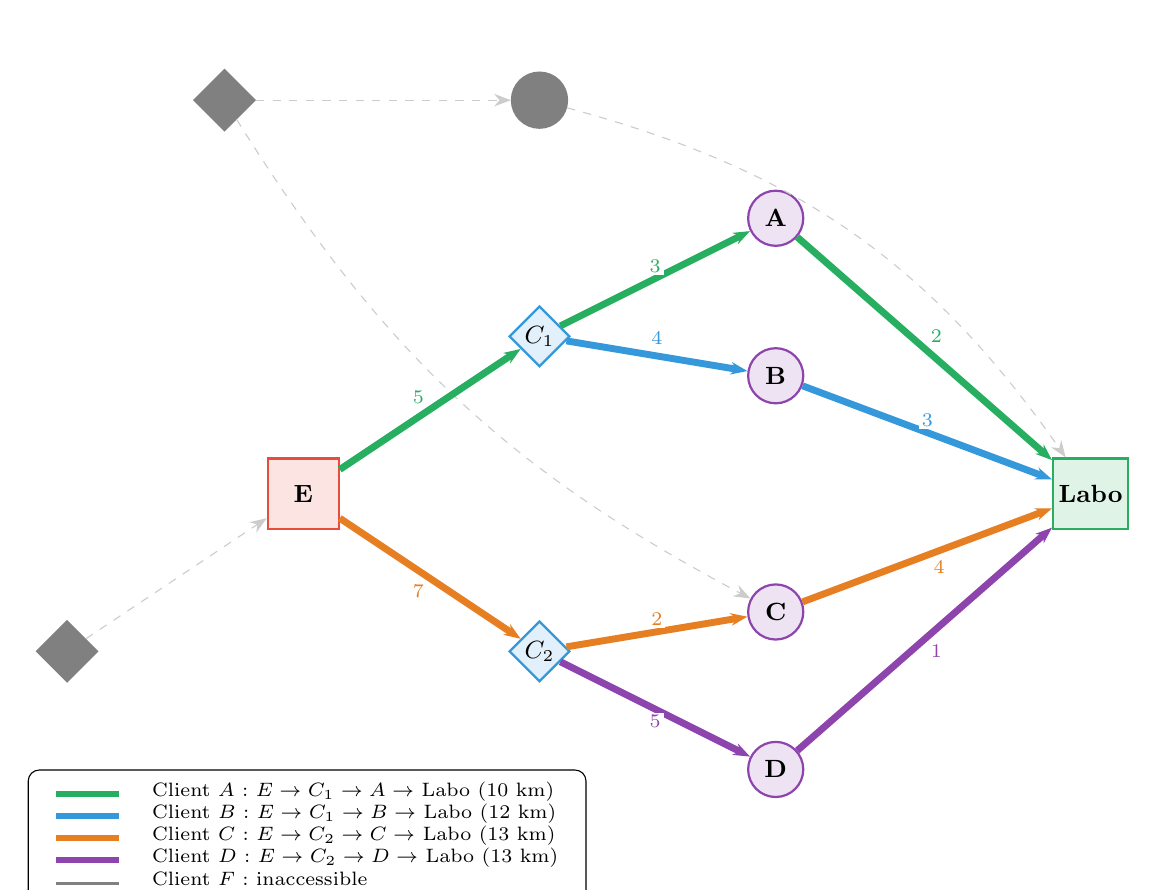
\begin{tikzpicture}[
  >={Stealth[length=6pt]},
  entrepot/.style={rectangle,draw=critcolor,fill=critcolor!15,thick,
                   minimum size=0.9cm,font=\small\bfseries,inner sep=2pt},
  cuisine/.style={diamond,draw=starcolor,fill=starcolor!15,thick,
                  minimum size=0.7cm,font=\small\bfseries,inner sep=1pt},
  client/.style={circle,draw=pathD,fill=pathD!15,thick,
                 minimum size=0.7cm,font=\small\bfseries,inner sep=1pt},
  labo/.style={rectangle,draw=acpmcolor,fill=acpmcolor!15,thick,
               minimum size=0.9cm,font=\small\bfseries,inner sep=2pt},
  arcfaint/.style={->,thin,gray!40,dashed},
  pathArc/.style={->,line width=2.5pt},
  lbl/.style={font=\scriptsize,fill=white,inner sep=1pt}
]
\node[entrepot] (E)  at (0,0)    {E};
\node[cuisine]  (C1) at (3,2)    {$C_1$};
\node[cuisine]  (C2) at (3,-2)   {$C_2$};
\node[cuisine,gray] (C3) at (-1,5)   {$C_3$};
\node[cuisine,gray] (C4) at (-3,-2)  {$C_4$};
\node[client]   (A)  at (6,3.5)  {A};
\node[client]   (B)  at (6,1.5)  {B};
\node[client]   (C)  at (6,-1.5) {C};
\node[client]   (D)  at (6,-3.5) {D};
\node[client,gray] (F)  at (3,5)    {F};
\node[labo]     (L)  at (10,0)   {Labo};
\draw[arcfaint] (C3) -- (F);
\draw[arcfaint] (C3) to[bend right=15] (C);
\draw[arcfaint] (C4) -- (E);
\draw[arcfaint] (F)  to[bend left=20] (L);
\draw[pathArc,pathA] (E)  -- node[lbl,above left]{5}   (C1);
\draw[pathArc,pathA] (C1) -- node[lbl,above]{3}        (A);
\draw[pathArc,pathA] (A)  -- node[lbl,above right]{2}  (L);
\draw[pathArc,pathB] (C1) -- node[lbl,above=2pt]{4}    (B);
\draw[pathArc,pathB] (B)  -- node[lbl,above]{3}        (L);
\draw[pathArc,pathC] (E)  -- node[lbl,below left]{7}   (C2);
\draw[pathArc,pathC] (C2) -- node[lbl,above]{2}        (C);
\draw[pathArc,pathC] (C)  -- node[lbl,below right]{4}  (L);
\draw[pathArc,pathD] (C2) -- node[lbl,below]{5}        (D);
\draw[pathArc,pathD] (D)  -- node[lbl,below right]{1}  (L);
\node[draw,rounded corners,fill=white,anchor=north west,inner sep=4pt,font=\scriptsize] at (-3.5,-3.5) {
  \begin{tabular}{ll}
  \textcolor{pathA}{\rule{0.8cm}{2pt}} & Client $A$ : $E\to C_1\to A\to$ Labo (10 km)\\
  \textcolor{pathB}{\rule{0.8cm}{2pt}} & Client $B$ : $E\to C_1\to B\to$ Labo (12 km)\\
  \textcolor{pathC}{\rule{0.8cm}{2pt}} & Client $C$ : $E\to C_2\to C\to$ Labo (13 km)\\
  \textcolor{pathD}{\rule{0.8cm}{2pt}} & Client $D$ : $E\to C_2\to D\to$ Labo (13 km)\\
  \textcolor{gray}{\rule{0.8cm}{1pt}}  & Client $F$ : inaccessible
  \end{tabular}
};
\end{tikzpicture}
}
\captionof{figure}{Plus courts chemins obtenus par l'algorithme de Dijkstra}
\end{center}

\subsubsection{Synthèse des trajets}

\begin{center}\small
\begin{tabular}{c|c|c|c}
\toprule
\textbf{Client} & \textbf{Chemin} & \textbf{Distance (km)} & \textbf{Accessible}\\
\midrule
$A$ & $E\to C_1\to A\to$ Labo & \textbf{10} & Oui\\
$B$ & $E\to C_1\to B\to$ Labo & \textbf{12} & Oui\\
$C$ & $E\to C_2\to C\to$ Labo & \textbf{13} & Oui\\
$D$ & $E\to C_2\to D\to$ Labo & \textbf{13} & Oui\\
$F$ & — & $+\infty$ & \textcolor{critcolor}{Non}\\
\bottomrule
\end{tabular}
\end{center}

\begin{resultbox}
\textbf{Conclusion.} La cuisine $C_1$ dessert les clients les plus proches du
laboratoire ($A$ et $B$) et constitue donc le \textbf{nœud logistique le plus
efficace}. Le client $F$ nécessite l'ajout d'un arc orienté $E \to C_3$ pour
être desservi.
\end{resultbox}

\newpage

% ─────────────────────────────────────────────────────────────────────────
\subsection{Arbre Couvrant de Poids Minimal — Kruskal}
% ─────────────────────────────────────────────────────────────────────────

\subsubsection{Application de l'algorithme de Kruskal}

L'algorithme trie les $\binom{10}{2}=45$ arêtes par poids croissant, puis ajoute chaque
arête à condition qu'elle ne forme pas de cycle (vérifié par Union-Find). L'algorithme
s'arrête après $n-1 = 9$ arêtes sélectionnées.

\begin{center}\small
\rowcolors{2}{acpmcolor!8}{white}
\begin{tabular}{clccl}
\toprule
\textbf{Ordre} & \textbf{Arête} & \textbf{Poids (km)} & \textbf{Cumulé} & \textbf{Décision}\\
\midrule
1 & $A - B$       & 2 & 2  & Acceptée (1\textsuperscript{re} composante)\\
2 & $C_2 - C$     & 2 & 4  & Acceptée (nouvelle composante)\\
3 & $C - D$       & 3 & 7  & Acceptée (étend $\{C_2,C\}$)\\
4 & $C_1 - A$     & 3 & 10 & Acceptée (étend $\{A,B\}$)\\
5 & $C_1 - C_2$   & 4 & 14 & Acceptée (fusionne 2 composantes)\\
6 & $C_4 - C$     & 4 & 18 & Acceptée (raccroche $C_4$)\\
7 & $E - C_1$     & 5 & 23 & Acceptée (raccroche $E$)\\
8 & $C_2 - C_3$   & 6 & 29 & Acceptée (raccroche $C_3$)\\
9 & $C_3 - F$     & 6 & \textbf{35} & Acceptée (raccroche $F$ — fin)\\
\bottomrule
\end{tabular}
\end{center}

\subsubsection{Visualisation de l'ACPM obtenu}

\begin{center}
\resizebox{0.85\textwidth}{!}{%
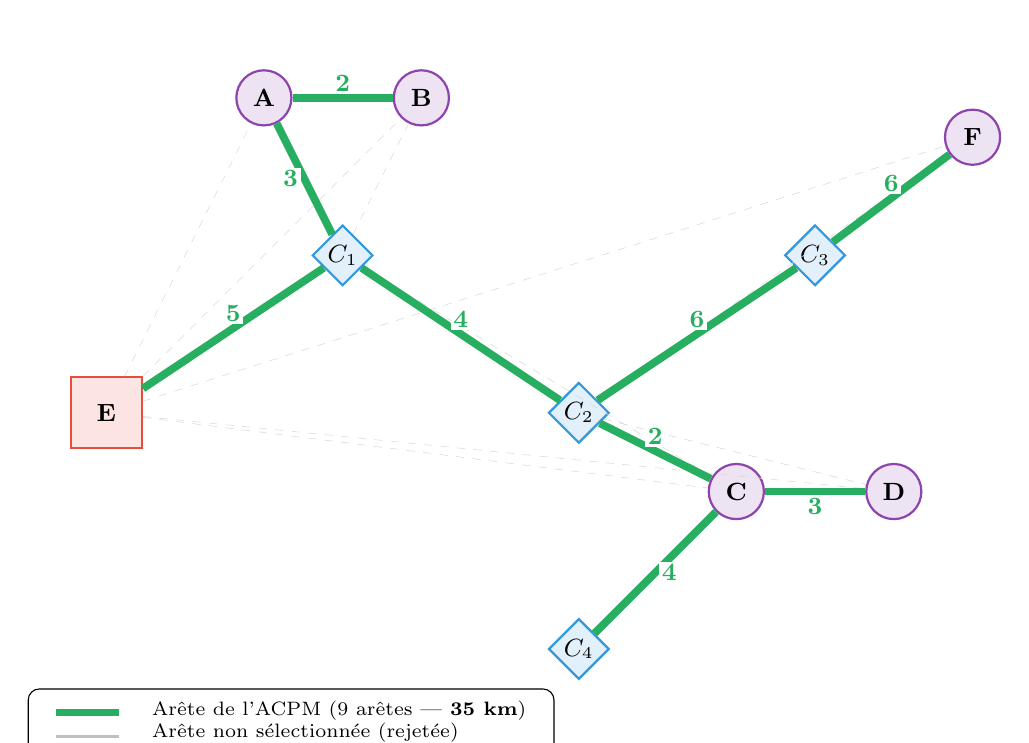
\begin{tikzpicture}[
  entrepot/.style={rectangle,draw=critcolor,fill=critcolor!15,thick,
                   minimum size=0.9cm,font=\small\bfseries,inner sep=2pt},
  cuisine/.style={diamond,draw=starcolor,fill=starcolor!15,thick,
                  minimum size=0.7cm,font=\small\bfseries,inner sep=1pt},
  client/.style={circle,draw=pathD,fill=pathD!15,thick,
                 minimum size=0.7cm,font=\small\bfseries,inner sep=1pt},
  acpm/.style={line width=2.8pt,acpmcolor},
  rejected/.style={very thin,gray!30,dashed},
  lbl/.style={font=\small,fill=white,inner sep=1pt,font=\small\bfseries}
]
\node[entrepot] (E)  at (-3,0)   {E};
\node[cuisine]  (C1) at (0,2)    {$C_1$};
\node[cuisine]  (C2) at (3,0)    {$C_2$};
\node[cuisine]  (C3) at (6,2)    {$C_3$};
\node[cuisine]  (C4) at (3,-3)   {$C_4$};
\node[client]   (A)  at (-1,4)   {A};
\node[client]   (B)  at (1,4)    {B};
\node[client]   (C)  at (5,-1)   {C};
\node[client]   (D)  at (7,-1)   {D};
\node[client]   (F)  at (8,3.5)  {F};
\draw[rejected] (E)--(A); \draw[rejected] (E)--(B);
\draw[rejected] (E)--(C); \draw[rejected] (E)--(D);
\draw[rejected] (E)--(F); \draw[rejected] (C2)--(D);
\draw[rejected] (C2)--(F); \draw[rejected] (C1)--(B);
\draw[rejected] (C1)--(C);
\draw[acpm] (A)  -- node[lbl,above]{2}   (B);
\draw[acpm] (C2) -- node[lbl,above]{2}   (C);
\draw[acpm] (C)  -- node[lbl,below]{3}   (D);
\draw[acpm] (C1) -- node[lbl,left]{3}    (A);
\draw[acpm] (C1) -- node[lbl,above]{4}   (C2);
\draw[acpm] (C4) -- node[lbl,right]{4}   (C);
\draw[acpm] (E)  -- node[lbl,above]{5}   (C1);
\draw[acpm] (C2) -- node[lbl,above]{6}   (C3);
\draw[acpm] (C3) -- node[lbl,above]{6}   (F);
\node[draw,rounded corners,fill=white,anchor=north west,inner sep=4pt,font=\scriptsize] at (-4,-3.5) {
  \begin{tabular}{ll}
  \textcolor{acpmcolor}{\rule{0.8cm}{2.5pt}} & Arête de l'ACPM (9 arêtes — \textbf{35 km})\\
  \textcolor{gray!50}{\rule{0.8cm}{1pt}}     & Arête non sélectionnée (rejetée)
  \end{tabular}
};
\end{tikzpicture}
}
\captionof{figure}{Arbre Couvrant de Poids Minimal obtenu par Kruskal — total : \textbf{35 km}}
\end{center}

\begin{resultbox}
\textbf{Conclusion.} L'ACPM relie les 10 sites avec seulement \textbf{35 km} de fibre
optique, contre \textbf{120 km} pour une étoile depuis $E$. L'économie est de
\textbf{85 km, soit 70,8\,\%}. L'ACPM exploite les proximités locales ($A$--$B$=2 km,
$C_2$--$C$=2 km, $C$--$D$=3 km, $C_1$--$A$=3 km) plutôt que de rayonner depuis l'entrepôt.
\end{resultbox}

\newpage

% ─────────────────────────────────────────────────────────────────────────
\subsection{Ordonnancement PERT}
% ─────────────────────────────────────────────────────────────────────────

\subsubsection{Tableau PERT — dates et marges}

\begin{center}\small
\setlength{\tabcolsep}{4pt}
\begin{tabular}{clccccccc}
\toprule
\textbf{Tâche} & \textbf{Description} & $d_i$ & $ES$ & $EF$ & $LS$ & $LF$ & $MT$ & \textbf{Critique}\\
\midrule
$P_1$ & Pesée                & 20 & 0   & 20  & 0   & 20  & \cellcolor{critcolor!25}\textbf{0} & \cellcolor{critcolor!25}Oui\\
$P_2$ & Cuisson              & 40 & 20  & 60  & 20  & 60  & \cellcolor{critcolor!25}\textbf{0} & \cellcolor{critcolor!25}Oui\\
$P_3$ & Assaisonnement       & 15 & 60  & 75  & 60  & 75  & \cellcolor{critcolor!25}\textbf{0} & \cellcolor{critcolor!25}Oui\\
$P_4$ & Conditionnement      & 30 & 75  & 105 & 75  & 105 & \cellcolor{critcolor!25}\textbf{0} & \cellcolor{critcolor!25}Oui\\
$L_1$ & Chargement camion    & 10 & 105 & 115 & 105 & 115 & \cellcolor{critcolor!25}\textbf{0} & \cellcolor{critcolor!25}Oui\\
$L_2$ & Livraison client A   & 12 & 115 & 127 & 121 & 133 & 6 & Non\\
$L_3$ & Livraison client B   & 18 & 115 & 133 & 115 & 133 & \cellcolor{critcolor!25}\textbf{0} & \cellcolor{critcolor!25}Oui\\
$L_4$ & Retour laboratoire   & 25 & 133 & 158 & 133 & 158 & \cellcolor{critcolor!25}\textbf{0} & \cellcolor{critcolor!25}Oui\\
\bottomrule
\end{tabular}
\end{center}

\medskip
\noindent\textbf{Durée totale} : 158 min (fin à 10h38)\quad
\textbf{Chemin critique} : $P_1\to P_2\to P_3\to P_4\to L_1\to L_3\to L_4$

\subsubsection{Diagramme PERT (méthode potentiels-étapes)}

Chaque sommet (cercle) représente un \textbf{événement}. Le format du nœud est :
\begin{center}
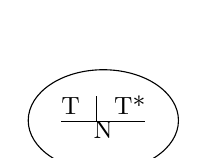
\begin{tikzpicture}[scale=0.8]
\node[draw,ellipse,inner sep=4pt,font=\small]
  {\renewcommand{\arraystretch}{0.7}\begin{tabular}{@{}c|c@{}}T&T*\\\hline\multicolumn{2}{@{}c@{}}{N}\end{tabular}};
\end{tikzpicture}
\end{center}
où $T$ = date au plus tôt, $T^*$ = date au plus tard, $N$ = numéro de l'événement.
Les arcs portent le nom et la durée de la tâche : $\text{Tâche}(d_i)$.

\begin{center}
\resizebox{\textwidth}{!}{%
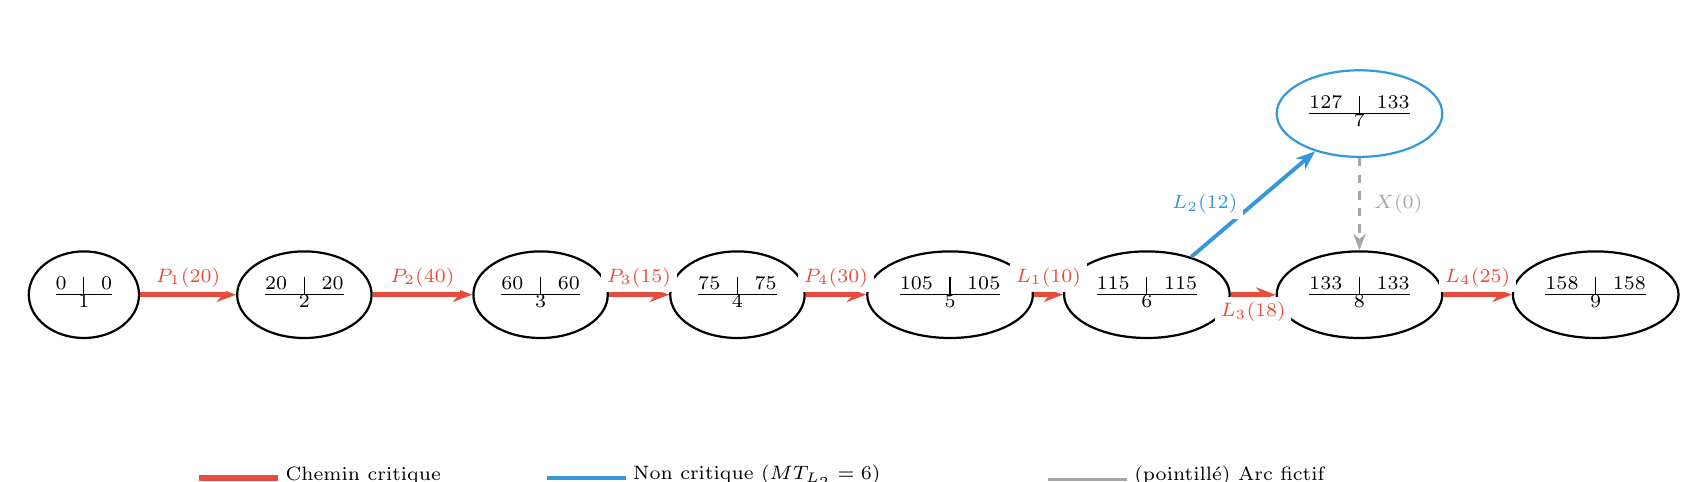
\begin{tikzpicture}[
  event/.style={ellipse,draw=black,thick,inner sep=3pt,font=\scriptsize,
                minimum width=1.4cm,minimum height=1.1cm},
  crit/.style={-{Stealth[length=7pt]},line width=1.6pt,critcolor},
  noncrit/.style={-{Stealth[length=7pt]},line width=1.4pt,starcolor},
  fictive/.style={-{Stealth[length=6pt]},dashed,thick,gray!70},
  lbl/.style={font=\scriptsize\bfseries,fill=white,inner sep=2pt}
]
\node[event] (n1) at (0,0)
  {\renewcommand{\arraystretch}{0.7}\begin{tabular}{@{}c|c@{}}0&0\\\hline\multicolumn{2}{@{}c@{}}{1}\end{tabular}};
\node[event] (n2) at (2.8,0)
  {\renewcommand{\arraystretch}{0.7}\begin{tabular}{@{}c|c@{}}20&20\\\hline\multicolumn{2}{@{}c@{}}{2}\end{tabular}};
\node[event] (n3) at (5.8,0)
  {\renewcommand{\arraystretch}{0.7}\begin{tabular}{@{}c|c@{}}60&60\\\hline\multicolumn{2}{@{}c@{}}{3}\end{tabular}};
\node[event] (n4) at (8.3,0)
  {\renewcommand{\arraystretch}{0.7}\begin{tabular}{@{}c|c@{}}75&75\\\hline\multicolumn{2}{@{}c@{}}{4}\end{tabular}};
\node[event] (n5) at (11,0)
  {\renewcommand{\arraystretch}{0.7}\begin{tabular}{@{}c|c@{}}105&105\\\hline\multicolumn{2}{@{}c@{}}{5}\end{tabular}};
\node[event] (n6) at (13.5,0)
  {\renewcommand{\arraystretch}{0.7}\begin{tabular}{@{}c|c@{}}115&115\\\hline\multicolumn{2}{@{}c@{}}{6}\end{tabular}};
\node[event,draw=starcolor] (n7) at (16.2,2.3)
  {\renewcommand{\arraystretch}{0.7}\begin{tabular}{@{}c|c@{}}127&133\\\hline\multicolumn{2}{@{}c@{}}{7}\end{tabular}};
\node[event] (n8) at (16.2,0)
  {\renewcommand{\arraystretch}{0.7}\begin{tabular}{@{}c|c@{}}133&133\\\hline\multicolumn{2}{@{}c@{}}{8}\end{tabular}};
\node[event] (n9) at (19.2,0)
  {\renewcommand{\arraystretch}{0.7}\begin{tabular}{@{}c|c@{}}158&158\\\hline\multicolumn{2}{@{}c@{}}{9}\end{tabular}};
\draw[crit] (n1) -- node[lbl,above]{$P_1(20)$} (n2);
\draw[crit] (n2) -- node[lbl,above]{$P_2(40)$} (n3);
\draw[crit] (n3) -- node[lbl,above]{$P_3(15)$} (n4);
\draw[crit] (n4) -- node[lbl,above]{$P_4(30)$} (n5);
\draw[crit] (n5) -- node[lbl,above]{$L_1(10)$} (n6);
\draw[crit] (n6) -- node[lbl,below]{$L_3(18)$} (n8);
\draw[crit] (n8) -- node[lbl,above]{$L_4(25)$} (n9);
\draw[noncrit] (n6) -- node[lbl,left,xshift=-3pt]{$L_2(12)$} (n7);
\draw[fictive] (n7) -- node[lbl,right,xshift=3pt]{$X(0)$} (n8);
\node[font=\scriptsize] at (3,-2.3) {\textcolor{critcolor}{\rule{1cm}{2pt}} Chemin critique};
\node[font=\scriptsize] at (8,-2.3) {\textcolor{starcolor}{\rule{1cm}{1.4pt}} Non critique ($MT_{L_2}=6$)};
\node[font=\scriptsize] at (14,-2.3) {\textcolor{gray!70}{\rule{1cm}{0.8pt}} (pointillé) Arc fictif};
\end{tikzpicture}
}
\captionof{figure}{Diagramme PERT — 9 événements, chemin critique en rouge \cite{cours4GI_ordonnancement}}
\end{center}

\begin{alertbox}
La \textbf{tâche fictive $X$} (durée 0) relie l'événement 7 (fin de $L_2$) à l'événement 8 ;
elle modélise la précédence «\,$L_4$ attend $L_2$ \emph{et} $L_3$\,». La marge de
$L_2$ se lit alors directement : $MT_{L_2} = T_8^* - T_6 - d_{L_2} = 133 - 115 - 12 = 6$ min.
\end{alertbox}

\subsubsection{Diagramme de Gantt}

\begin{center}
\resizebox{\textwidth}{!}{%
\begin{ganttchart}[
  hgrid,vgrid,
  x unit=0.08cm,
  y unit title=0.55cm,
  y unit chart=0.62cm,
  title height=1,
  title label font=\tiny,
  bar label font=\tiny\bfseries,
  bar label node/.append style={left=0.1cm},
  bar height=0.55,
  bar top shift=0.225,
  time slot format=simple,
  today=90,
  today rule/.style={orange!90!black,dashed,thick},
  today label={\tiny 9h30},
  today label font=\tiny\bfseries,
  today label node/.append style={above=0.08cm}
]{0}{160}
\gantttitle{\textbf{Temps (min depuis 8h00)}}{160}\\
\gantttitlelist[title label font=\tiny]{0,20,40,60,80,100,120,140,160}{20}\\
\ganttbar[bar/.append style={fill=critcolor!80,draw=critcolor!50}]{$P_1$ — Pesée (20 min)}{0}{19}\\
\ganttbar[bar/.append style={fill=critcolor!80,draw=critcolor!50}]{$P_2$ — Cuisson (40 min)}{20}{59}\\
\ganttbar[bar/.append style={fill=critcolor!80,draw=critcolor!50}]{$P_3$ — Assaisonnement (15 min)}{60}{74}\\
\ganttbar[bar/.append style={fill=critcolor!80,draw=critcolor!50}]{$P_4$ — Conditionnement (30 min)}{75}{104}\\
\ganttbar[bar/.append style={fill=critcolor!80,draw=critcolor!50}]{$L_1$ — Chargement (10 min)}{105}{114}\\
\ganttbar[bar/.append style={fill=starcolor!70,draw=starcolor!50}]{$L_2$ — Livraison A (12 min, MT=6)}{115}{126}\\
\ganttbar[bar/.append style={fill=critcolor!80,draw=critcolor!50}]{$L_3$ — Livraison B (18 min)}{115}{132}\\
\ganttbar[bar/.append style={fill=critcolor!80,draw=critcolor!50}]{$L_4$ — Retour Labo (25 min)}{133}{157}
\end{ganttchart}
}
\end{center}

\begin{warnbox}
Durée totale : \textbf{158 min} (fin à 10h38). Le deadline 9h30 (90 min) est dépassé de
\textbf{68 min}. Les tâches $L_2$ et $L_3$ \textbf{démarrent simultanément} à $t=115$ min
(2 livreurs) — elles occupent des \textbf{lignes séparées} dans le Gantt et ne se
superposent pas.
\end{warnbox}

\newpage

% ─────────────────────────────────────────────────────────────────────────
\subsection{Programmation linéaire — Méthode du Simplexe}
% ─────────────────────────────────────────────────────────────────────────

Conformément aux notations du cours ($\max Z = cx$, $Ax \leq b$, $x \geq 0$),
les tableaux du simplexe présentent : le membre de droite ($b_i$) à l'extrême
gauche, les variables ($x_1, x_2, \ldots, x_{n+m}$) au centre, et la variable
de base à l'extrême droite. La ligne $Z$ figure en tête du tableau.

\subsubsection{Étape 1 — Variables et fonction objectif}

Les variables de décision sont $x_1 = S$ (Standard), $x_2 = V$ (Végétarien),
$x_3 = G$ (sans Gluten), avec $c_1=3$, $c_2=4$, $c_3=5$ (\texteuro/repas).

\noindent$\max\; Z = 3x_1 + 4x_2 + 5x_3$,\quad soit la ligne $Z$ : $Z - 3x_1 - 4x_2 - 5x_3 = 0$.

\subsubsection{Étape 2 — Changement de variables (bornes inférieures)}

Posons $x_1' = x_1-20$, $x_2' = x_2-20$, $x_3' = x_3-20$ ($x_j' \geq 0$).
La fonction objectif devient $Z' = 3x_1' + 4x_2' + 5x_3'$, avec $Z = Z'+240$.

\subsubsection{Étape 3 — Forme standard}

Les variables d'écart $x_4, \ldots, x_{12}$ transforment chaque inégalité en
égalité. La numérotation suit la convention du cours ($x_{n+i}$, $i=1\ldots m$) :

\begin{center}\small
\begin{tabular}{ll|ll}
$x_4$ : écart légumes   & $x_5$ : écart viande    &
$x_6$ : écart céréales  & $x_7$ : écart cuisson \\
$x_8$ : écart MO        & $x_9$ : écart total     &
$x_{10}$ : écart $x_1'\leq 80$ & $x_{11}$ : écart $x_2'\leq 60$ \\
$x_{12}$ : écart $x_3'\leq 30$ & & &
\end{tabular}
\end{center}

Base initiale : $\{x_4, x_5, x_6, x_7, x_8, x_9, x_{10}, x_{11}, x_{12}\}$.

\subsubsection{Étape 4 — Tableaux du simplexe}

\noindent\textit{Conventions :}\quad
\colorbox{pivotcol}{\strut colonne pivot}\quad
\colorbox{pivotrow}{\strut ligne pivot}\quad
\colorbox{pivotelt}{\strut\textbf{pivot}}\quad
Ligne $Z$ en tête — membre de droite à gauche — variable de base à droite.

\begin{landscape}
\thispagestyle{fancy}
\vspace*{0.3cm}

\begin{center}
\textbf{Tableau T\textsubscript{0} — Initial}\\[2pt]
\textit{Var. entrante : $x_3'$ (coeff. $-5$, plus négatif de $L_0$).
Var. sortante : $x_{12}$ (ratio min $= 30/1 = 30$). Pivot $= 1$.}

\vspace{0.3cm}
\setlength{\tabcolsep}{3pt}
\renewcommand{\arraystretch}{1.3}
\scriptsize
\resizebox{\linewidth}{!}{%
\begin{tabular}{|c|c|c|>{\columncolor{pivotcol}}c|c|c|c|c|c|c|c|c|c|c|}
\hline
$b$ & $x_1'$ & $x_2'$ & $x_3'$ &
$x_4$ & $x_5$ & $x_6$ & $x_7$ & $x_8$ & $x_9$ & $x_{10}$ & $x_{11}$ & $x_{12}$ &
\textbf{V.B.} \\
\hline
0   & \textcolor{critcolor}{$-3$} & \textcolor{critcolor}{$-4$} & \textcolor{critcolor}{$-5$}
    & 0 & 0 & 0 & 0 & 0 & 0 & 0 & 0 & 0 & $Z$ \\
\hline
64  & 0,5 & 1   & 0,3 & 1 & 0 & 0 & 0 & 0 & 0 & 0 & 0 & 0 & $x_4$     \\
64  & 0,8 & 0   & 0   & 0 & 1 & 0 & 0 & 0 & 0 & 0 & 0 & 0 & $x_5$     \\
82  & 0,4 & 0,6 & 0,9 & 0 & 0 & 1 & 0 & 0 & 0 & 0 & 0 & 0 & $x_6$     \\
350 & 2   & 1,5 & 3   & 0 & 0 & 0 & 1 & 0 & 0 & 0 & 0 & 0 & $x_7$     \\
506 & 1,5 & 1,2 & 2   & 0 & 0 & 0 & 0 & 1 & 0 & 0 & 0 & 0 & $x_8$     \\
140 & 1   & 1   & 1   & 0 & 0 & 0 & 0 & 0 & 1 & 0 & 0 & 0 & $x_9$     \\
80  & 1   & 0   & 0   & 0 & 0 & 0 & 0 & 0 & 0 & 1 & 0 & 0 & $x_{10}$  \\
60  & 0   & 1   & 0   & 0 & 0 & 0 & 0 & 0 & 0 & 0 & 1 & 0 & $x_{11}$  \\
\rowcolor{pivotrow}
\textbf{30} & 0 & 0 & \cellcolor{pivotelt}\textbf{1}
  & 0 & 0 & 0 & 0 & 0 & 0 & 0 & 0 & 1 & $x_{12}$ $\leftarrow$ \\
\hline
\end{tabular}
}
\end{center}

\vspace{0.4cm}

\begin{center}
\textbf{Tableau T\textsubscript{1} — Après pivot : $x_3'$ entre, $x_{12}$ sort}\quad ($Z'=150$)\\[2pt]
\textit{Var. entrante : $x_2'$ (coeff. $-4$). Var. sortante : $x_4$ (ratio $55/1=55$). Pivot $=1$.}

\vspace{0.3cm}
\setlength{\tabcolsep}{3pt}
\renewcommand{\arraystretch}{1.3}
\scriptsize
\resizebox{\linewidth}{!}{%
\begin{tabular}{|c|c|>{\columncolor{pivotcol}}c|c|c|c|c|c|c|c|c|c|c|c|}
\hline
$b$ & $x_1'$ & $x_2'$ & $x_3'$ &
$x_4$ & $x_5$ & $x_6$ & $x_7$ & $x_8$ & $x_9$ & $x_{10}$ & $x_{11}$ & $x_{12}$ &
\textbf{V.B.} \\
\hline
150 & \textcolor{critcolor}{$-3$} & \textcolor{critcolor}{$-4$} & 0
  & 0 & 0 & 0 & 0 & 0 & 0 & 0 & 0 & 5 & $Z$ \\
\hline
\rowcolor{pivotrow}
\textbf{55}  & 0,5 & \cellcolor{pivotelt}\textbf{1} & 0
  & 1 & 0 & 0 & 0 & 0 & 0 & 0 & 0 & $-0{,}3$ & $x_4$ $\leftarrow$ \\
64  & 0,8 & 0   & 0 & 0 & 1 & 0 & 0 & 0 & 0 & 0 & 0 & 0        & $x_5$    \\
55  & 0,4 & 0,6 & 0 & 0 & 0 & 1 & 0 & 0 & 0 & 0 & 0 & $-0{,}9$ & $x_6$    \\
260 & 2   & 1,5 & 0 & 0 & 0 & 0 & 1 & 0 & 0 & 0 & 0 & $-3$     & $x_7$    \\
446 & 1,5 & 1,2 & 0 & 0 & 0 & 0 & 0 & 1 & 0 & 0 & 0 & $-2$     & $x_8$    \\
110 & 1   & 1   & 0 & 0 & 0 & 0 & 0 & 0 & 1 & 0 & 0 & $-1$     & $x_9$    \\
80  & 1   & 0   & 0 & 0 & 0 & 0 & 0 & 0 & 0 & 1 & 0 & 0        & $x_{10}$ \\
60  & 0   & 1   & 0 & 0 & 0 & 0 & 0 & 0 & 0 & 0 & 1 & 0        & $x_{11}$ \\
30  & 0   & 0   & 1 & 0 & 0 & 0 & 0 & 0 & 0 & 0 & 0 & 1        & $x_3'$   \\
\hline
\end{tabular}
}
\end{center}

\end{landscape}

\begin{landscape}
\thispagestyle{fancy}
\vspace*{0.3cm}

\begin{center}
\textbf{Tableau T\textsubscript{2} — Après pivot : $x_2'$ entre, $x_4$ sort}\quad ($Z'=370$)\\[2pt]
\textit{Var. entrante : $x_1'$ (coeff. $-1$). Var. sortante : $x_{10}$ (ratio $80/1=80$). Pivot $=1$.}

\vspace{0.3cm}
\setlength{\tabcolsep}{3pt}
\renewcommand{\arraystretch}{1.3}
\scriptsize
\resizebox{\linewidth}{!}{%
\begin{tabular}{|c|>{\columncolor{pivotcol}}c|c|c|c|c|c|c|c|c|c|c|c|c|}
\hline
$b$ & $x_1'$ & $x_2'$ & $x_3'$ &
$x_4$ & $x_5$ & $x_6$ & $x_7$ & $x_8$ & $x_9$ & $x_{10}$ & $x_{11}$ & $x_{12}$ &
\textbf{V.B.} \\
\hline
370 & \textcolor{critcolor}{$-1$} & 0 & 0
  & 4 & 0 & 0 & 0 & 0 & 0 & 0 & 0 & 3,8 & $Z$ \\
\hline
55    & 0,5  & 1 & 0 & 1        & 0 & 0 & 0 & 0 & 0 & 0 & 0 & $-0{,}3$  & $x_2'$   \\
64    & 0,8  & 0 & 0 & 0        & 1 & 0 & 0 & 0 & 0 & 0 & 0 & 0         & $x_5$    \\
22    & 0,1  & 0 & 0 & $-0{,}6$ & 0 & 1 & 0 & 0 & 0 & 0 & 0 & $-0{,}72$ & $x_6$    \\
177,5 & 1,25 & 0 & 0 & $-1{,}5$ & 0 & 0 & 1 & 0 & 0 & 0 & 0 & $-2{,}55$ & $x_7$    \\
380   & 0,9  & 0 & 0 & $-1{,}2$ & 0 & 0 & 0 & 1 & 0 & 0 & 0 & $-1{,}64$ & $x_8$    \\
55    & 0,5  & 0 & 0 & $-1$     & 0 & 0 & 0 & 0 & 1 & 0 & 0 & $-0{,}7$  & $x_9$    \\
\rowcolor{pivotrow}
\textbf{80} & \cellcolor{pivotelt}\textbf{1} & 0 & 0
  & 0 & 0 & 0 & 0 & 0 & 0 & 1 & 0 & 0 & $x_{10}$ $\leftarrow$ \\
5     & $-0{,}5$ & 0 & 0 & $-1$ & 0 & 0 & 0 & 0 & 0 & 0 & 1 & $0{,}3$ & $x_{11}$ \\
30    & 0 & 0 & 1 & 0 & 0 & 0 & 0 & 0 & 0 & 0 & 0 & $-1$ & $x_3'$   \\
\hline
\end{tabular}
}
\end{center}

\vspace{0.4cm}

\begin{center}
\textbf{Tableau T\textsubscript{3} — Après pivot : $x_1'$ entre, $x_{10}$ sort}\quad ($Z'=450$)\\[2pt]
\textcolor{acpmcolor}{\textbf{Tous les coeff. de la ligne $Z$ sont $\geq 0$ $\Rightarrow$ solution optimale.}}

\vspace{0.3cm}
\setlength{\tabcolsep}{3pt}
\renewcommand{\arraystretch}{1.3}
\scriptsize
\resizebox{\linewidth}{!}{%
\begin{tabular}{|c|c|c|c|c|c|c|c|c|c|c|c|c|c|}
\hline
$b$ & $x_1'$ & $x_2'$ & $x_3'$ &
$x_4$ & $x_5$ & $x_6$ & $x_7$ & $x_8$ & $x_9$ & $x_{10}$ & $x_{11}$ & $x_{12}$ &
\textbf{V.B.} \\
\hline
\textbf{450} & 0 & 0 & 0 & 4 & 0 & 0 & 0 & 0 & 0 & 1 & 0 & 3,8 & $Z$ \\
\hline
\textbf{15}   & 0 & 1 & 0 & 1        & 0 & 0 & 0 & 0 & 0 & $-0{,}5$ & 0 & $-0{,}3$  & $x_2'$   \\
\textbf{0}    & 0 & 0 & 0 & 0        & 1 & 0 & 0 & 0 & 0 & $-0{,}8$ & 0 & 0         & $x_5$    \\
\textbf{14}   & 0 & 0 & 0 & $-0{,}6$ & 0 & 1 & 0 & 0 & 0 & $-0{,}1$ & 0 & $-0{,}72$ & $x_6$    \\
\textbf{77,5} & 0 & 0 & 0 & $-1{,}5$ & 0 & 0 & 1 & 0 & 0 & $-1{,}25$& 0 & $-2{,}55$ & $x_7$    \\
\textbf{308}  & 0 & 0 & 0 & $-1{,}2$ & 0 & 0 & 0 & 1 & 0 & $-0{,}9$ & 0 & $-1{,}64$ & $x_8$    \\
\textbf{15}   & 0 & 0 & 0 & $-1$     & 0 & 0 & 0 & 0 & 1 & $-0{,}5$ & 0 & $-0{,}7$  & $x_9$    \\
\textbf{80}   & 1 & 0 & 0 & 0        & 0 & 0 & 0 & 0 & 0 & 1        & 0 & 0         & $x_1'$   \\
\textbf{45}   & 0 & 0 & 0 & $-1$     & 0 & 0 & 0 & 0 & 0 & 0,5      & 1 & 0,3       & $x_{11}$ \\
\textbf{30}   & 0 & 0 & 1 & 0        & 0 & 0 & 0 & 0 & 0 & 0        & 0 & $-1$      & $x_3'$   \\
\hline
\end{tabular}
}
\end{center}

\end{landscape}

\subsubsection{Étape 5 — Interprétation et solution optimale}

\noindent\textbf{Lecture du tableau T\textsubscript{3} :}
\[
x_1' = 80,\quad x_2' = 15,\quad x_3' = 30,\quad Z' = 450
\]

\noindent\textbf{Retour aux variables originales :}
\[
x_1 = x_1' + 20 = 100,\quad x_2 = x_2' + 20 = 35,\quad x_3 = x_3' + 20 = 50
\]

\noindent\textbf{Valeur de la fonction objectif :}
\[
Z = Z' + 240 = 450 + 240 = \boxed{690 \;\text{\texteuro}/\text{jour}}
\]

\begin{resultbox}
\textbf{Solution optimale :} produire chaque jour
\begin{itemize}[noitemsep]
  \item $\boxed{x_1 = S = 100}$ repas Standard \quad (apport : $3 \times 100 = 300$ \texteuro)
  \item $\boxed{x_2 = V = 35}$ repas Végétariens \quad (apport : $4 \times 35 = 140$ \texteuro)
  \item $\boxed{x_3 = G = 50}$ repas Sans Gluten \quad (apport : $5 \times 50 = 250$ \texteuro)
\end{itemize}
\textbf{Marge totale maximale : 690 \texteuro/jour}, sur 185 repas produits (sur 200 max).

\medskip
\noindent\textbf{Contraintes saturées} ($x_{n+i} = 0$, variable d'écart nulle) :
\begin{itemize}[noitemsep]
  \item $x_4 = 0$ : contrainte des \textbf{légumes} (64 kg après substitution) saturée ;
  \item $x_5 = 0$ : contrainte de la \textbf{viande} (64 kg après substitution) saturée ;
  \item $x_{10} = 0$ : borne $x_1' \leq 80$ ($x_1 = 100$) saturée ;
  \item $x_{12} = 0$ : borne $x_3' \leq 30$ ($x_3 = 50$) saturée.
\end{itemize}
Les ressources céréales, cuisson, MO et capacité totale ne sont pas limitantes.
\end{resultbox}

\newpage

% =========================================================================
\section{Analyse de sensibilité}
% =========================================================================

\subsection{Comparaison des distances $E \to \text{Labo}$ via chaque client}

Le tableau récapitule, pour chaque client, le plus court chemin depuis l'entrepôt $E$
jusqu'au laboratoire de contrôle qualité, tel que calculé par l'algorithme de Dijkstra
sur le graphe orienté.

\begin{center}\small
\begin{tabular}{ccccl}
\toprule
\textbf{Client} & \textbf{Chemin emprunté} & \textbf{Détail (km)} & \textbf{Total} & \textbf{Cuisine}\\
\midrule
$A$ & $E\to C_1\to A\to$ Labo & $5+3+2$ & \textbf{10 km} & $C_1$\\
$B$ & $E\to C_1\to B\to$ Labo & $5+4+3$ & \textbf{12 km} & $C_1$\\
$C$ & $E\to C_2\to C\to$ Labo & $7+2+4$ & \textbf{13 km} & $C_2$\\
$D$ & $E\to C_2\to D\to$ Labo & $7+5+1$ & \textbf{13 km} & $C_2$\\
$F$ & Aucun chemin orienté depuis $E$ vers $C_3$ & — & — & —\\
\bottomrule
\end{tabular}
\end{center}

Le trajet le plus court est celui passant par le client $A$ (10 km), suivi du client $B$
(12 km), tous deux desservis par la cuisine satellite $C_1$ depuis l'entrepôt. Les clients
$C$ et $D$, rattachés à $C_2$, affichent la même distance totale de 13 km malgré des
arcs internes différents : l'arc $C_2 \to D$ est plus long (5 km contre 2 km pour
$C_2 \to C$), mais l'arc $D \to$ Labo est nettement plus court (1 km contre 4 km), ce
qui compense exactement l'écart.

D'un point de vue stratégique, $C_1$ dessert les clients les plus proches du laboratoire
et constitue le \textbf{nœud logistique le plus efficace}. Quant au client $F$, dépendant
de $C_3$ qui n'a aucun arc entrant depuis $E$, sa livraison ne peut pas être modélisée
sans ajout d'arcs supplémentaires dans le graphe \cite{cours4GI_graphes}.

% ─────────────────────────────────────────────────────────────────────────
\subsection{ACPM versus réseau en étoile depuis $E$}
% ─────────────────────────────────────────────────────────────────────────

\begin{center}\small
\rowcolors{2}{blue!4}{white}
\begin{tabular}{lcc}
\toprule
\textbf{Critère} & \textbf{Étoile depuis $E$} & \textbf{ACPM (Kruskal)}\\
\midrule
Nombre d'arêtes               & 9 & 9\\
Longueur totale               & 120 km & \textbf{35 km}\\
Arête la plus longue          & 22 km ($E$--$F$) & 6 km ($C_3$--$F$)\\
Nœud central                  & $E$ (degré 9) & $C_1, C_2, C$ (degrés $\leq 4$)\\
\midrule
\textbf{Économie ACPM}        & \multicolumn{2}{c}{\textbf{85 km, soit 70,8\,\% de réduction}}\\
\bottomrule
\end{tabular}
\end{center}

\medskip

La solution en étoile repose sur une hypothèse implicite erronée : elle suppose que
l'entrepôt $E$ est géographiquement central par rapport à tous les sites. Or la matrice
des distances révèle que ce n'est pas le cas --- $E$ est certes proche de $C_1$ (5 km)
et de $C_2$ (7 km), mais très éloigné des clients finaux (14 km de $A$, 18 km de $C$,
20 km de $D$, jusqu'à 22 km de $F$). Tirer un câble direct depuis $E$ vers chacun de
ces sites revient donc à ignorer les fortes proximités locales existant entre certains
nœuds.

L'algorithme de Kruskal exploite précisément ces proximités. Par exemple, relier $A$
à $B$ ne coûte que 2 km, alors que les deux liaisons en étoile ($E$--$A$ et $E$--$B$)
auraient coûté $14+13=27$ km au total. De même, la chaîne $C_2 \to C \to D$ représente
$2+3=5$ km contre $7+5=12$ km pour relier $E$ à $C$ et $E$ à $D$ séparément. Ce
principe se généralise à l'ensemble du réseau et conduit à une réduction de
\textbf{70,8\,\%} de la longueur totale câblée \cite{cours4GI_graphes}.

\begin{alertbox}
\textbf{Limite de l'ACPM.} L'arbre couvrant ne garantit qu'un seul chemin entre deux
nœuds. En cas de rupture d'un câble, le réseau se partitionne en deux composantes
déconnectées, là où l'étoile ne priverait qu'un seul site. Dans un contexte
opérationnel, SmartFood pourrait ajouter une ou deux arêtes supplémentaires à l'ACPM
pour sécuriser les connexions les plus critiques, au prix d'un surcoût limité.
\end{alertbox}

% ─────────────────────────────────────────────────────────────────────────
\subsection{Impact d'un second livreur}
% ─────────────────────────────────────────────────────────────────────────

\begin{center}\small
\begin{tabular}{lcc}
\toprule
\textbf{Critère} & \textbf{S1 — 1 livreur (séquentiel)} & \textbf{S2 — 2 livreurs (parallèle)}\\
\midrule
Durée totale                  & 170 min (10h50) & \textbf{158 min (10h38)}\\
Gain sur la durée             & — & \textbf{12 min (7,1\,\%)}\\
$MT_{L_2}$                    & 0 (critique)    & 6 min\\
Nombre de tâches critiques    & 8 (toutes)      & 7 (sauf $L_2$)\\
Chemin critique               & $\cdots\to L_1\to L_2\to L_3\to L_4$
                              & $\cdots\to L_1\to L_3\to L_4$\\
\bottomrule
\end{tabular}
\end{center}

\medskip

Avec un seul livreur (scénario S1), $L_2$ et $L_3$ sont exécutées séquentiellement et
\textbf{toutes} les tâches se retrouvent sur le chemin critique ; la moindre
perturbation se répercute immédiatement sur la date de fin de projet. Avec deux
livreurs (scénario S2), $L_2$ et $L_3$ démarrent simultanément à $t = 115$ min (dès
la fin de $L_1$). La tâche $L_2$, plus courte (12 min contre 18 min pour $L_3$), se
termine en avance et dégage une \textbf{marge totale de 6 min} :
\[
MT_{L_2} = LS_{L_2} - ES_{L_2} = 121 - 115 = 6 \text{ min.}
\]
Cette marge offre à l'équipe de livraison du client $A$ une flexibilité précieuse face
aux aléas (trafic, indisponibilité momentanée du client) sans remettre en cause la date
de fin globale.

Le gain de 12 minutes est cependant \textbf{plafonné par la durée de $L_3$} (18 min) :
c'est elle qui dicte la date de début de $L_4$, et non $L_2$. Pour réduire davantage
la durée totale, il faudrait soit comprimer $L_3$, soit introduire d'autres
parallélisations en amont --- par exemple, chevaucher partiellement $P_2$ (cuisson) et
$P_3$ (assaisonnement) si les équipements le permettent
\cite{cours4GI_ordonnancement}.

\begin{warnbox}
\textbf{Rappel sur le deadline.} Même avec deux livreurs, le projet se termine à
\textbf{10h38}, soit un dépassement de \textbf{68 min} par rapport au deadline de
9h30. Le second livreur n'est donc pas suffisant à lui seul. Les actions prioritaires
portent sur le chemin critique amont, notamment $P_2$ (cuisson, 40 min) dont la durée
représente 25\,\% de la durée totale du projet.
\end{warnbox}

\newpage

% =========================================================================
\section*{Conclusion}
\addcontentsline{toc}{section}{Conclusion}
% =========================================================================

Ce projet autour du cas SmartFood nous a permis d'aborder de manière concrète quatre
grandes problématiques de la recherche opérationnelle, en les appliquant à un scénario
logistique réaliste et cohérent.

Sur le plan des \textbf{plus courts chemins}, l'algorithme de Dijkstra a permis
d'identifier pour chaque client le trajet optimal depuis l'entrepôt jusqu'au laboratoire
de contrôle. Les résultats mettent en évidence des disparités significatives selon les
cuisines utilisées, et soulignent l'intérêt d'une affectation intelligente des commandes
aux cuisines satellites les mieux positionnées géographiquement.

L'\textbf{arbre couvrant de poids minimal} obtenu par l'algorithme de Kruskal représente
une solution de câblage fibre optique nettement plus économique qu'une simple étoile
rayonnant depuis l'entrepôt central. Cette approche illustre l'efficacité des méthodes
gloutonnières pour ce type de problème combinatoire.

L'\textbf{ordonnancement PERT} a révélé un chemin critique traversant les étapes de
production, de chargement et de livraison, laissant peu de marges sur la séquence
principale. L'analyse avec un délai imposé à 9h30 a montré la nécessité d'intervenir sur
des tâches spécifiques, et l'ajout d'un second livreur permettrait de réduire sensiblement
la durée totale en parallélisant les livraisons.

Enfin, la \textbf{programmation linéaire} a fourni une solution de production maximisant
la marge quotidienne dans le respect des contraintes de ressources et de demande. Une
analyse de sensibilité sur les coefficients de la fonction objectif et les disponibilités
des ressources permettrait à l'entreprise d'anticiper les impacts de variations
d'approvisionnement ou de politique tarifaire.

En définitive, ce travail démontre que les outils d'optimisation offrent à SmartFood —
comme à toute entreprise logistique — des leviers concrets d'amélioration de la
performance. Des extensions naturelles pourraient inclure la prise en compte de
contraintes temporelles dynamiques, l'intégration d'une demande stochastique ou encore
la modélisation multi-objectifs pour arbitrer entre coût, délai et satisfaction client.



% =========================================================================
\newpage
\section*{Références bibliographiques}
\addcontentsline{toc}{section}{Références bibliographiques}
% =========================================================================

\renewcommand{\refname}{}
\vspace{-1.8em}
\begin{thebibliography}{9}

\bibitem{cours4GI_graphes}
Cours de Recherche Opérationnelle 4GI.
\textit{Chapitre~: Théorie des graphes --- représentations, plus courts
chemins (algorithme de Dijkstra), arbres couvrants de poids minimal
(algorithmes de Kruskal et Prim)}.
Support de cours, filière 4GI,
École Nationale Supérieure Polytechnique de Yaoundé,
Année universitaire 2025--2026.

\bibitem{cours4GI_ordonnancement}
Cours de Recherche Opérationnelle 4GI.
\textit{Chapitre~: Techniques d'ordonnancement des tâches ---
Diagramme de Gantt, méthode PERT (\emph{Program Evaluation and Research
Task}), méthode des Potentiels Métra (MPM), chemin critique, marges
totales et marges libres}.
Support de cours, filière 4GI,
École Nationale Supérieure Polytechnique de Yaoundé,
Année universitaire 2025--2026.

\bibitem{cours4GI_PL}
Cours de Recherche Opérationnelle 4GI.
\textit{Chapitre~: Programmation Linéaire --- modélisation, forme
standard, méthode du Simplexe (tableaux, pivotage, test d'optimalité),
méthode du Grand M, méthode des deux phases, analyse de sensibilité}.
Support de cours, filière 4GI,
École Nationale Supérieure Polytechnique de Yaoundé,
Année universitaire 2025--2026.

\end{thebibliography}

\newpage

% =========================================================================
\appendix
\section{Code Python commenté}
% =========================================================================

L'implémentation complète est organisée en quatre modules Python autonomes, intégrés
dans une application Streamlit pour la visualisation interactive.

\subsection{Module 1 — Dijkstra : plus courts chemins}

\begin{lstlisting}[caption={module\_dijkstra.py}]
import heapq
from collections import defaultdict

# ──────────────────────────────────────────────────────────────────────────
# Graphe orienté SmartFood (arcs et poids en km)
# ──────────────────────────────────────────────────────────────────────────
ARCS = [
    ('E','C1',5), ('E','C2',7),
    ('C1','A',3), ('C1','B',4),
    ('C2','C',2), ('C2','D',5),
    ('C3','F',6), ('C3','C',9),
    ('C4','E',8),
    ('A','Labo',2), ('B','Labo',3),
    ('C','Labo',4), ('D','Labo',1),
    ('F','Labo',7),
]

def construire_graphe(arcs):
    """Construit un dictionnaire d'adjacence depuis la liste d'arcs."""
    graph = defaultdict(dict)
    for u, v, w in arcs:
        graph[u][v] = w
    return graph

def dijkstra(graph, source):
    """Algorithme de Dijkstra avec tas binaire."""
    tous_noeuds = set(graph.keys()) | {v for u in graph for v in graph[u]}
    dist   = {n: float('inf') for n in tous_noeuds}
    parent = {n: None         for n in tous_noeuds}
    dist[source] = 0
    pq, finali = [(0, source)], set()
    while pq:
        d, u = heapq.heappop(pq)
        if u in finali:
            continue
        finali.add(u)
        for v, w in graph.get(u, {}).items():
            if d + w < dist[v]:
                dist[v]   = d + w
                parent[v] = u
                heapq.heappush(pq, (dist[v], v))
    return dist, parent

def reconstruire_chemin(parent, debut, fin):
    """Reconstruit le chemin depuis debut jusqu'a fin."""
    chemin, noeud = [], fin
    while noeud is not None:
        chemin.append(noeud)
        noeud = parent.get(noeud)
    chemin.reverse()
    return chemin if chemin and chemin[0] == debut else []

# ── Programme principal ────────────────────────────────────────────────
graph = construire_graphe(ARCS)
dist_E, parent_E = dijkstra(graph, 'E')

print("=== Plus courts chemins E -> client -> Labo ===")
for client in ['A', 'B', 'C', 'D', 'F']:
    d_e_c = dist_E.get(client, float('inf'))
    dist_c, par_c = dijkstra(graph, client)
    d_c_l = dist_c.get('Labo', float('inf'))
    if d_e_c < float('inf') and d_c_l < float('inf'):
        chemin = reconstruire_chemin(parent_E, 'E', client) + \
                 reconstruire_chemin(par_c, client, 'Labo')[1:]
        print(f"{client}: {' -> '.join(chemin)} = {d_e_c + d_c_l} km")
    else:
        print(f"{client}: INACCESSIBLE")
\end{lstlisting}

\subsection{Module 2 — Kruskal : ACPM fibre optique}

\begin{lstlisting}[caption={module\_kruskal.py}]
NOEUDS = ['E','C1','C2','C3','C4','A','B','C','D','F']
MATRICE = [
    [ 0,  5,  7, 12,  9, 14, 13, 18, 20, 22],
    [ 5,  0,  4, 10,  8,  3,  4, 11, 13, 15],
    [ 7,  4,  0,  6,  5,  9,  8,  2,  5, 12],
    [12, 10,  6,  0,  7, 15, 14,  9, 11,  6],
    [ 9,  8,  5,  7,  0, 12, 11,  4,  6, 10],
    [14,  3,  9, 15, 12,  0,  2, 10, 12, 16],
    [13,  4,  8, 14, 11,  2,  0,  9, 11, 15],
    [18, 11,  2,  9,  4, 10,  9,  0,  3,  8],
    [20, 13,  5, 11,  6, 12, 11,  3,  0,  7],
    [22, 15, 12,  6, 10, 16, 15,  8,  7,  0],
]

class UnionFind:
    """Structure Union-Find avec compression de chemin et union par rang."""
    def __init__(self, noeuds):
        self.parent = {n: n for n in noeuds}
        self.rang   = {n: 0 for n in noeuds}
    def trouver(self, x):
        if self.parent[x] != x:
            self.parent[x] = self.trouver(self.parent[x])
        return self.parent[x]
    def unir(self, x, y):
        rx, ry = self.trouver(x), self.trouver(y)
        if rx == ry:
            return False  # cycle detecte
        if self.rang[rx] < self.rang[ry]:
            rx, ry = ry, rx
        self.parent[ry] = rx
        if self.rang[rx] == self.rang[ry]:
            self.rang[rx] += 1
        return True

def kruskal(noeuds, matrice):
    """Construit l'ACPM par l'algorithme de Kruskal."""
    n = len(noeuds)
    aretes = sorted(
        [(matrice[i][j], noeuds[i], noeuds[j])
         for i in range(n) for j in range(i+1, n)],
        key=lambda x: x[0]
    )
    uf, acpm, total = UnionFind(noeuds), [], 0
    for poids, u, v in aretes:
        if uf.unir(u, v):
            acpm.append((u, v, poids))
            total += poids
            if len(acpm) == n - 1:
                break
    return acpm, total

acpm, total = kruskal(NOEUDS, MATRICE)
print(f"ACPM = {total} km")
for u, v, w in acpm:
    print(f"  {u} -- {v} : {w} km")
\end{lstlisting}

\subsection{Module 3 — PERT : ordonnancement}

\begin{lstlisting}[caption={module\_pert.py}]
TACHES = {
    'P1': {'dur': 20, 'pred': []},
    'P2': {'dur': 40, 'pred': ['P1']},
    'P3': {'dur': 15, 'pred': ['P2']},
    'P4': {'dur': 30, 'pred': ['P3']},
    'L1': {'dur': 10, 'pred': ['P4']},
    'L2': {'dur': 12, 'pred': ['L1']},
    'L3': {'dur': 18, 'pred': ['L1']},
    'L4': {'dur': 25, 'pred': ['L2','L3']},
}
ORDRE = ['P1','P2','P3','P4','L1','L2','L3','L4']

def calcul_pert(taches, ordre):
    """Calcule ES, EF, LS, LF, MT et le chemin critique."""
    ES, EF = {}, {}
    # Passage avant : dates au plus tot
    for t in ordre:
        ES[t] = max((EF[p] for p in taches[t]['pred']), default=0)
        EF[t] = ES[t] + taches[t]['dur']
    T_projet = max(EF.values())
    # Passage arriere : dates au plus tard
    LS, LF = {}, {}
    for t in reversed(ordre):
        succs = [s for s in ordre if t in taches[s]['pred']]
        LF[t] = min((LS[s] for s in succs), default=T_projet)
        LS[t] = LF[t] - taches[t]['dur']
    # Marges et chemin critique
    MT = {t: LS[t] - ES[t] for t in ordre}
    critique = [t for t in ordre if MT[t] == 0]
    return ES, EF, LS, LF, MT, critique, T_projet

ES, EF, LS, LF, MT, critique, T = calcul_pert(TACHES, ORDRE)
print(f"Duree totale : {T} min")
print(f"Chemin critique : {' -> '.join(critique)}")
\end{lstlisting}

\subsection{Module 4 — Programmation linéaire (simplexe)}

\begin{lstlisting}[caption={module\_lp.py}]
from scipy.optimize import linprog

# Changement de variables : S'=S-20, V'=V-20, G'=G-20
# Max Z' = 3S' + 4V' + 5G'  (+ 240 a la fin)
# scipy.linprog MINIMISE, donc on inverse : min -3S' -4V' -5G'
c_obj = [-3, -4, -5]

# Contraintes Ax <= b (apres substitution)
A_ub = [
    [0.5, 1.0, 0.3],    # legumes  <= 64
    [0.8, 0.0, 0.0],    # viande   <= 64
    [0.4, 0.6, 0.9],    # cereales <= 82
    [2.0, 1.5, 3.0],    # cuisson  <= 350
    [1.5, 1.2, 2.0],    # MO       <= 506
    [1.0, 1.0, 1.0],    # total    <= 140
]
b_ub = [64, 64, 82, 350, 506, 140]

# Bornes : S' in [0,80], V' in [0,60], G' in [0,30]
bornes = [(0, 80), (0, 60), (0, 30)]

res = linprog(c_obj, A_ub=A_ub, b_ub=b_ub, bounds=bornes, method='highs')
if res.success:
    Sp, Vp, Gp = res.x
    S, V, G    = Sp + 20, Vp + 20, Gp + 20  # variables originales
    Z = -res.fun + 240                       # objectif reel
    print(f"S = {S:.0f}, V = {V:.0f}, G = {G:.0f}")
    print(f"Marge totale = {Z:.2f} EUR/jour")
\end{lstlisting}


\end{document}